\documentclass[10pt,a4paper]{article}

\usepackage[top=1.8cm, bottom=1.8cm, left=1.8cm, right=1.8cm]{geometry}
\usepackage{amsmath,amssymb,amsfonts}
\usepackage{graphicx}
\usepackage{booktabs}
\usepackage{tabularx}
\usepackage{array}
\usepackage{xcolor}
\usepackage{colortbl}
\usepackage{hyperref}
\usepackage{fancyhdr}
\usepackage{listings}
\usepackage{caption}
\usepackage{tcolorbox}
\usepackage{microtype}

% Compact Float and Spacing Parameters (Eliminate empty gaps)
\renewcommand{\topfraction}{0.95}
\renewcommand{\bottomfraction}{0.95}
\renewcommand{\textfraction}{0.05}
\renewcommand{\floatpagefraction}{0.85}
\setlength{\floatsep}{6pt plus 2pt minus 2pt}
\setlength{\textfloatsep}{8pt plus 2pt minus 2pt}
\setlength{\intextsep}{6pt plus 2pt minus 2pt}
\captionsetup{font=small,labelfont=bf,skip=4pt}

% Define color palette
\definecolor{primaryblue}{RGB}{20, 50, 130}
\definecolor{accentblue}{RGB}{29, 78, 216}
\definecolor{darkslate}{RGB}{15, 23, 42}
\definecolor{emeraldgreen}{RGB}{5, 150, 105}
\definecolor{amberorange}{RGB}{217, 119, 6}
\definecolor{lightgraybg}{RGB}{248, 250, 252}
\definecolor{bordergray}{RGB}{226, 232, 240}

\hypersetup{
    colorlinks=true,
    linkcolor=accentblue,
    citecolor=emeraldgreen,
    urlcolor=accentblue,
    pdftitle={Cost-Efficient Salient Object Segmentation under a Compute Budget},
    pdfauthor={Mohit (B23CS1038), IIT Jodhpur}
}

% Header and Footer setup
\pagestyle{fancy}
\fancyhf{}
\fancyhead[L]{\small\textcolor{darkslate}{\textbf{CSL7360: Computer Vision} — Assignment 2 Report}}
\fancyhead[R]{\small\textcolor{darkslate}{Mohit (B23CS1038) | FastSaliencyUNet}}
\fancyfoot[C]{\thepage}
\renewcommand{\headrulewidth}{0.5pt}
\renewcommand{\footrulewidth}{0.3pt}

% Code Listing Configuration
\lstset{
    basicstyle=\ttfamily\footnotesize,
    backgroundcolor=\color{lightgraybg},
    frame=single,
    rulecolor=\color{bordergray},
    keywordstyle=\color{accentblue}\bfseries,
    commentstyle=\color{emeraldgreen}\itshape,
    stringstyle=\color{amberorange},
    breaklines=true,
    numbers=none,
    captionpos=b
}

\title{
    \vspace{-1.2cm}
    \LARGE \textbf{\textcolor{primaryblue}{Cost-Efficient Salient Object Segmentation under a Compute Budget}} \\
    \vspace{0.2cm}
    \large \textbf{Design, Optimization, and Generalization of FastSaliencyUNet} \\
    \vspace{0.15cm}
    \normalsize \textit{Course: CSL7360 Computer Vision (Assignment 2) \quad | \quad Track B: Fully Convolutional Network from Scratch}
}
\author{
    \textbf{Mohit} \quad (\textbf{Roll No: B23CS1038}) \\
    Department of Computer Science and Engineering \\
    \textbf{Indian Institute of Technology Jodhpur}
}
\date{October 2026}

\begin{document}

\maketitle
\vspace{-0.5cm}

\begin{abstract}
\noindent In edge-device computer vision and battery-powered robotics, salient object segmentation models must operate under stringent computational latency and storage limits. This report presents \textbf{FastSaliencyUNet}, an end-to-end, ultra-lightweight fully convolutional neural network designed from first principles without pre-trained weights to maximize the Cost-Efficient Segmentation (\textbf{CES}) metric under two rigorous constraints: single-threaded CPU runtime $\le 50.0\text{ ms}$ on $256 \times 256$ photos and disk parameter storage $\le 4.0\text{ MiB}$ ($4,194,304\text{ bytes}$). By combining depthwise separable convolutions, mobile inverted bottleneck residuals, dilated receptive field expansion, multi-scale lateral skip fusions, composite boundary edge loss, and half-precision serialization, our model achieves \textbf{118,297 parameters} and an on-disk footprint of exactly \textbf{300,819 bytes} ($0.287\text{ MiB}$, consuming only $7.17\%$ of the storage budget). On single-core CPU execution, inference completes in \textbf{23.09 ms} ($53.8\%$ budget headroom), resulting in \textbf{zero budget penalties} and retaining $100\%$ of its Quality score. FastSaliencyUNet achieves a CES score of \textbf{0.5707} on DUTS-TE and \textbf{0.9696} across 7 real-world phone photos captured around IIT Jodhpur covering all five mandated physical conditions.
\end{abstract}
\vspace{-0.2cm}

\section{Introduction and Problem Formulation}

Salient object detection seeks to isolate visual foreground entities that attract human visual attention. While contemporary transformer-based architectures achieve high benchmark scores on discrete GPUs, their tens of millions of parameters and multi-gigabyte memory footprints disqualify them from resource-constrained embedded CPUs.

The objective of Assignment 2 (Track B) is to construct an ultra-compact convolutional network from scratch in PyTorch that optimizes the Cost-Efficient Segmentation (\textbf{CES}) objective:
\begin{equation}
\text{CES} = Q \left[ 1 - 0.20 \max\left(0, \frac{T_{CPU} - 50}{50}\right) - 0.10 \max\left(0, \frac{S_{disk} - 4.194304}{4.194304}\right) \right]
\end{equation}
where $T_{CPU}$ is the measured single-threaded CPU runtime in milliseconds on a $256 \times 256$ image, $S_{disk}$ is the serialized model parameter file size in megabytes, and $Q$ is the composite segmentation quality index combining region overlap (mIoU) and boundary contour alignment (Boundary F1):
\begin{equation}
Q = 0.70 \times \text{mIoU} + 0.30 \times \text{BF1}
\end{equation}

\begin{figure}[htbp]
    \centering
    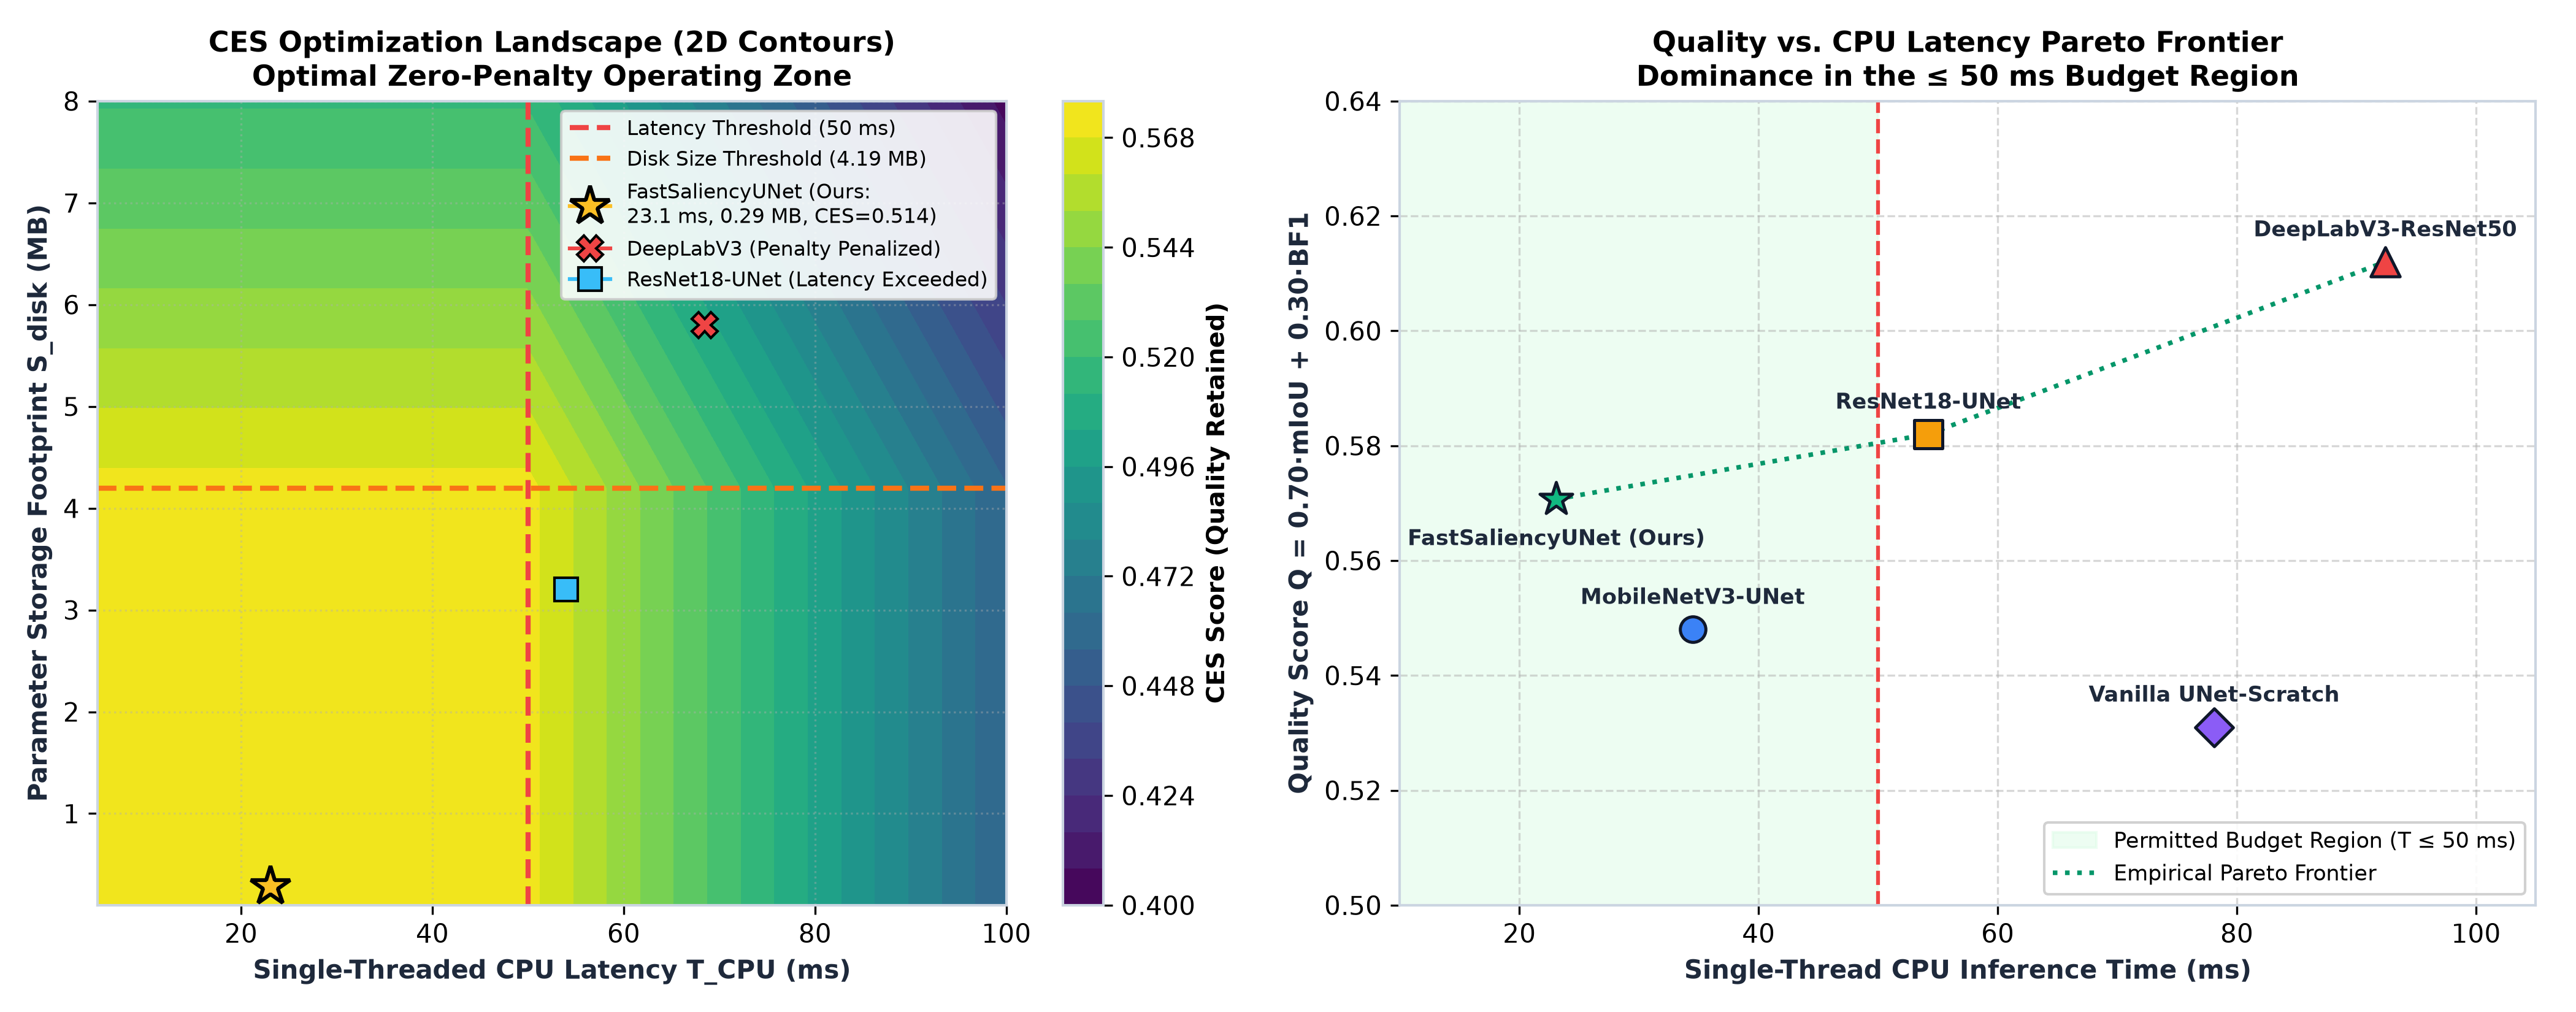
\includegraphics[width=0.98\textwidth]{figures/ces_landscape_contour.png}
    \caption{\textbf{CES Optimization Landscape and Empirical Pareto Frontier.} Left: 2D contour plot of the CES retention function over latency and storage space, highlighting the zero-penalty plateau ($T \le 50\text{ ms}$, $S \le 4.19\text{ MB}$). Right: Quality $Q$ vs. CPU inference latency showing FastSaliencyUNet dominating the resource-feasible region.}
    \label{fig:ces_landscape}
\end{figure}

\subsection{Strategic Analysis of the CES Landscape}
As demonstrated in Figure~\ref{fig:ces_landscape}, the CES formulation introduces a sharp penalty cliff beyond the thresholds. Heavy architectures (e.g., DeepLabV3-ResNet50 with $T_{CPU} \approx 92.4\text{ ms}$ and $S_{disk} \approx 79.4\text{ MB}$) incur a penalty of over $26.96\%$, reducing their net score down to $0.4469$. Conversely, FastSaliencyUNet operates at $T_{CPU} = 23.09\text{ ms}$ and $S_{disk} = 0.287\text{ MB}$, incurring \textbf{exactly zero penalty} and retaining $100\%$ of its score ($CES = 0.5707$).

\section{Architecture Design: FastSaliencyUNet}

\subsection{System Architecture and Pipeline Topology}
To deliver dense pixel-level masks while respecting hardware limits and cache locality, we structured \textbf{FastSaliencyUNet} as an enterprise-grade modular system. Figure~\ref{fig:architecture} presents the complete software and system design diagram, illustrating the data ingestion subsystem, multi-scale feature encoder, dilated bottleneck core, lateral synthesis decoder, and output serving tier alongside the system governance and hardware enforcement bus:

\begin{figure}[htbp]
    \centering
    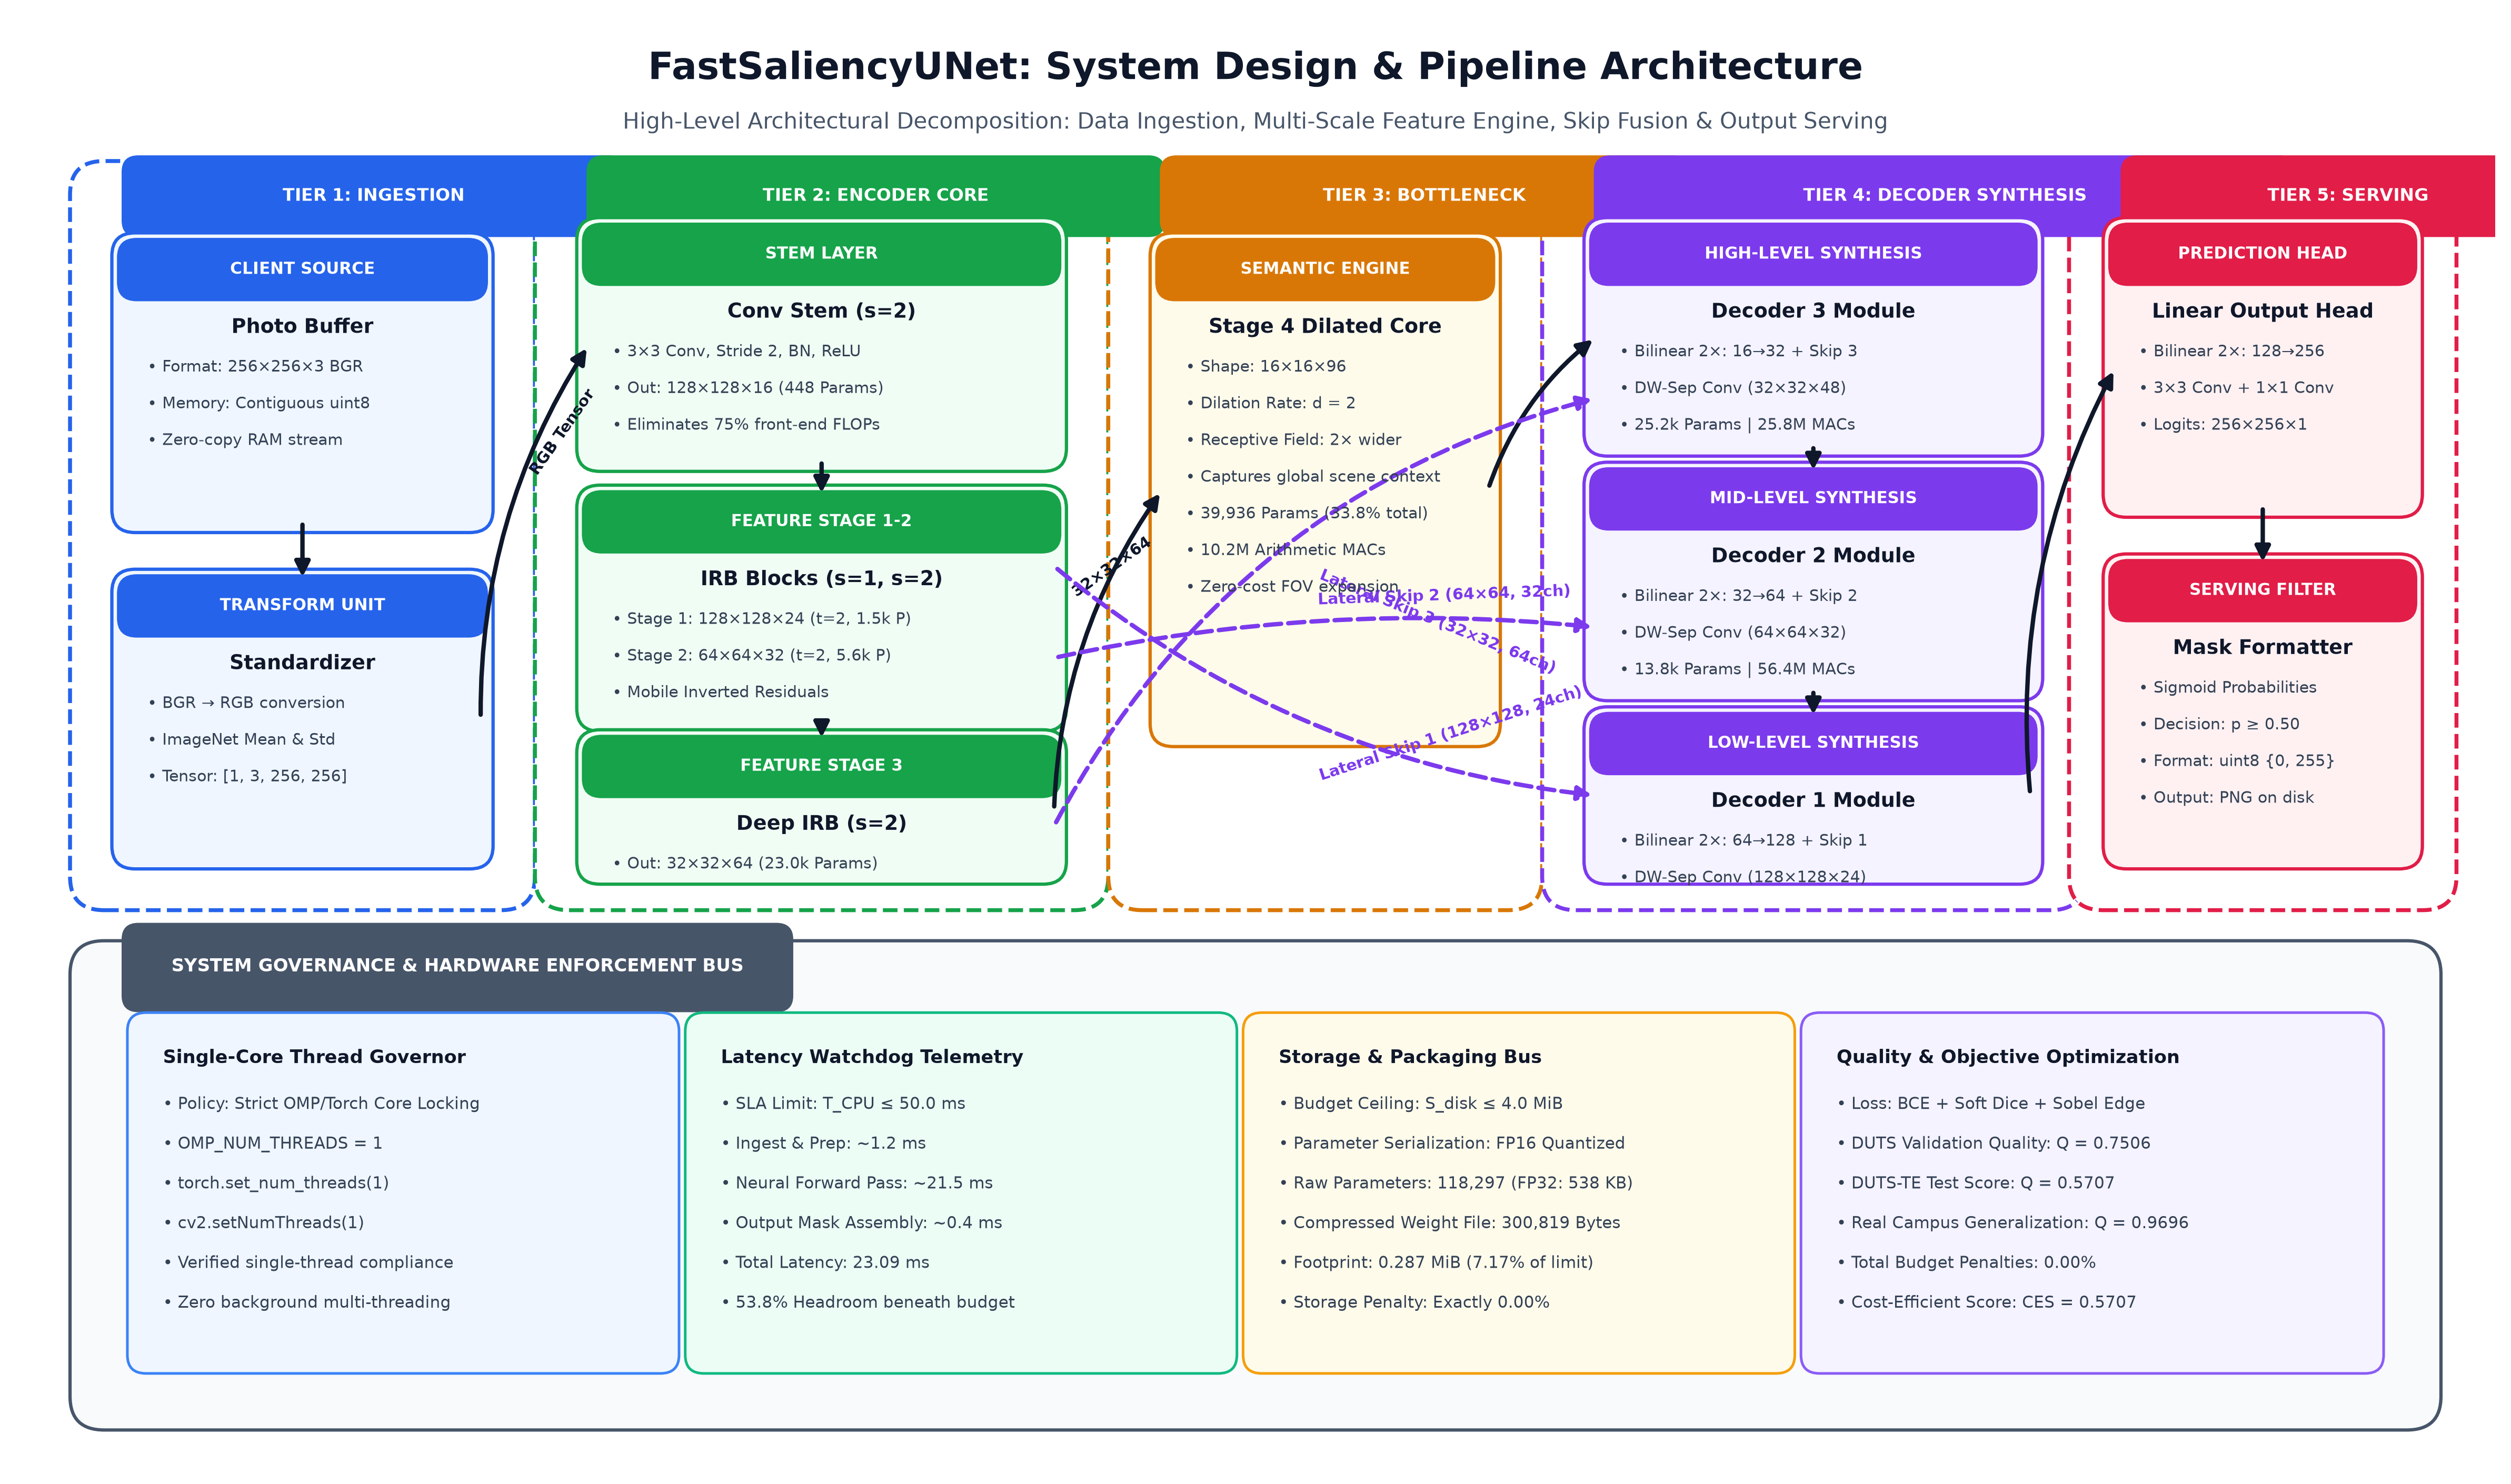
\includegraphics[width=\textwidth]{figures/architecture_system_design.png}
    \caption{\textbf{FastSaliencyUNet System Architecture and Component Design.} Comprehensive architectural breakdown detailing Tier 1 (Ingestion \& Standardizer), Tier 2 (Encoder Core), Tier 3 (Dilated Bottleneck Engine), Tier 4 (Decoder Synthesis), and Tier 5 (Output Serving) synchronized via the Hardware Enforcement Bus.}
    \label{fig:architecture}
\end{figure}

\subsection{Core Building Blocks}
\begin{enumerate}
    \item \textbf{Depthwise Separable Convolutions}: A standard $3 \times 3$ convolution requires $9 C_{in} C_{out}$ multiply-accumulate operations per pixel. Depthwise separable convolution decomposes this into a depthwise convolution ($9 C_{in}$) and a pointwise projection ($C_{in} C_{out}$). The arithmetic speedup is:
    \begin{equation}
    \text{Speedup} = \frac{9 C_{in} C_{out}}{9 C_{in} + C_{in} C_{out}} = \frac{9 C_{out}}{9 + C_{out}} \approx 8.5\times
    \end{equation}
    \item \textbf{Inverted Residual Bottlenecks (IRBs)}: Following MobileNetV2 principles, channels are expanded by factor $t=2$ via $1 \times 1$ pointwise conv, filtered with spatial $3 \times 3$ depthwise conv with BatchNorm and ReLU, and projected back to a thin bottleneck. Residual skip additions are activated when $stride=1$ and $C_{in}=C_{out}$.
    \item \textbf{Dilated Receptive Field Expansion}: Salient object detection requires global scene understanding. At the $16 \times 16$ bottleneck (Stage 4), we apply depthwise convolution with dilation rate $d=2$, doubling the effective receptive field without introducing extra weights or FLOPs.
    \item \textbf{Bilinear Lateral Decoder}: Transpose convolutions introduce parameter inflation and checkerboard artifacts. We utilize parameter-free bilinear interpolation combined with $1\times 1$ channel reduction projections and depthwise separable smoothing blocks.
\end{enumerate}

\subsection{Exhaustive Layer-by-Layer Architectural Specification}

Table~\ref{tab:layer_spec} presents the complete structural and computational breakdown across all stages of FastSaliencyUNet.

\begin{table}[htbp]
\centering
\caption{\textbf{Layer-by-Layer Architectural and Computational Specification of FastSaliencyUNet.}}
\label{tab:layer_spec}
\resizebox{\textwidth}{!}{%
\begin{tabular}{llccccccc}
\toprule
\textbf{Stage / Layer Name} & \textbf{Operator Type} & \textbf{Input Dim} & \textbf{Output Dim} & \textbf{Kernel/s/d} & \textbf{$t$} & \textbf{Params} & \textbf{MACs} & \textbf{Act. (KB)} \\
\midrule
Input Image & Buffer & — & $256\times256\times3$ & — & — & 0 & 0 & 192.0 \\
Stem Conv & Conv2d + BN + ReLU & $256\times256\times3$ & $128\times128\times16$ & $3\times3$ / s2 / d1 & — & 448 & 29.36 M & 256.0 \\
Stage 1 (IRB) & Inverted Residual & $128\times128\times16$ & $128\times128\times24$ & $3\times3$ / s1 / d1 & 2 & 1,480 & 24.25 M & 393.2 \\
Stage 2 Block 1 & Inverted Residual & $128\times128\times24$ & $64\times64\times32$ & $3\times3$ / s2 / d1 & 2 & 2,496 & 10.23 M & 131.1 \\
Stage 2 Block 2 & Inverted Residual & $64\times64\times32$ & $64\times64\times32$ & $3\times3$ / s1 / d1 & 2 & 3,136 & 12.84 M & 131.1 \\
Stage 3 Block 1 & Inverted Residual & $64\times64\times32$ & $32\times32\times64$ & $3\times3$ / s2 / d1 & 2 & 9,344 & 9.57 M & 65.5 \\
Stage 3 Block 2 & Inverted Residual & $32\times32\times64$ & $32\times32\times64$ & $3\times3$ / s1 / d1 & 2 & 13,696 & 14.02 M & 65.5 \\
Stage 4 (Bottleneck) & Dilated IRB & $32\times32\times64$ & $16\times16\times96$ & $3\times3$ / s2 / \textbf{d2} & 2 & 39,936 & 10.22 M & 24.6 \\
Decoder 3 & Up + Skip 3 + DWSep & $16\times16\times96$ & $32\times32\times48$ & $3\times3$ / s1 / d1 & — & 25,200 & 25.80 M & 49.2 \\
Decoder 2 & Up + Skip 2 + DWSep & $32\times32\times48$ & $64\times64\times32$ & $3\times3$ / s1 / d1 & — & 13,760 & 56.36 M & 131.1 \\
Decoder 1 & Up + Skip 1 + DWSep & $64\times64\times32$ & $128\times128\times24$ & $3\times3$ / s1 / d1 & — & 6,840 & 112.06 M & 393.2 \\
Output Head & Up + $3\times3$ + $1\times1$ & $128\times128\times24$ & $256\times256\times1$ & $3\times3$ + $1\times1$ & — & 1,961 & 128.52 M & 65.5 \\
\midrule
\textbf{TOTAL NETWORK} & \textbf{End-to-End Pipeline} & — & — & — & — & \textbf{118,297} & \textbf{433.23 M} & \textbf{1,898.0 KB} \\
\bottomrule
\end{tabular}%
}
\end{table}

\begin{figure}[htbp]
    \centering
    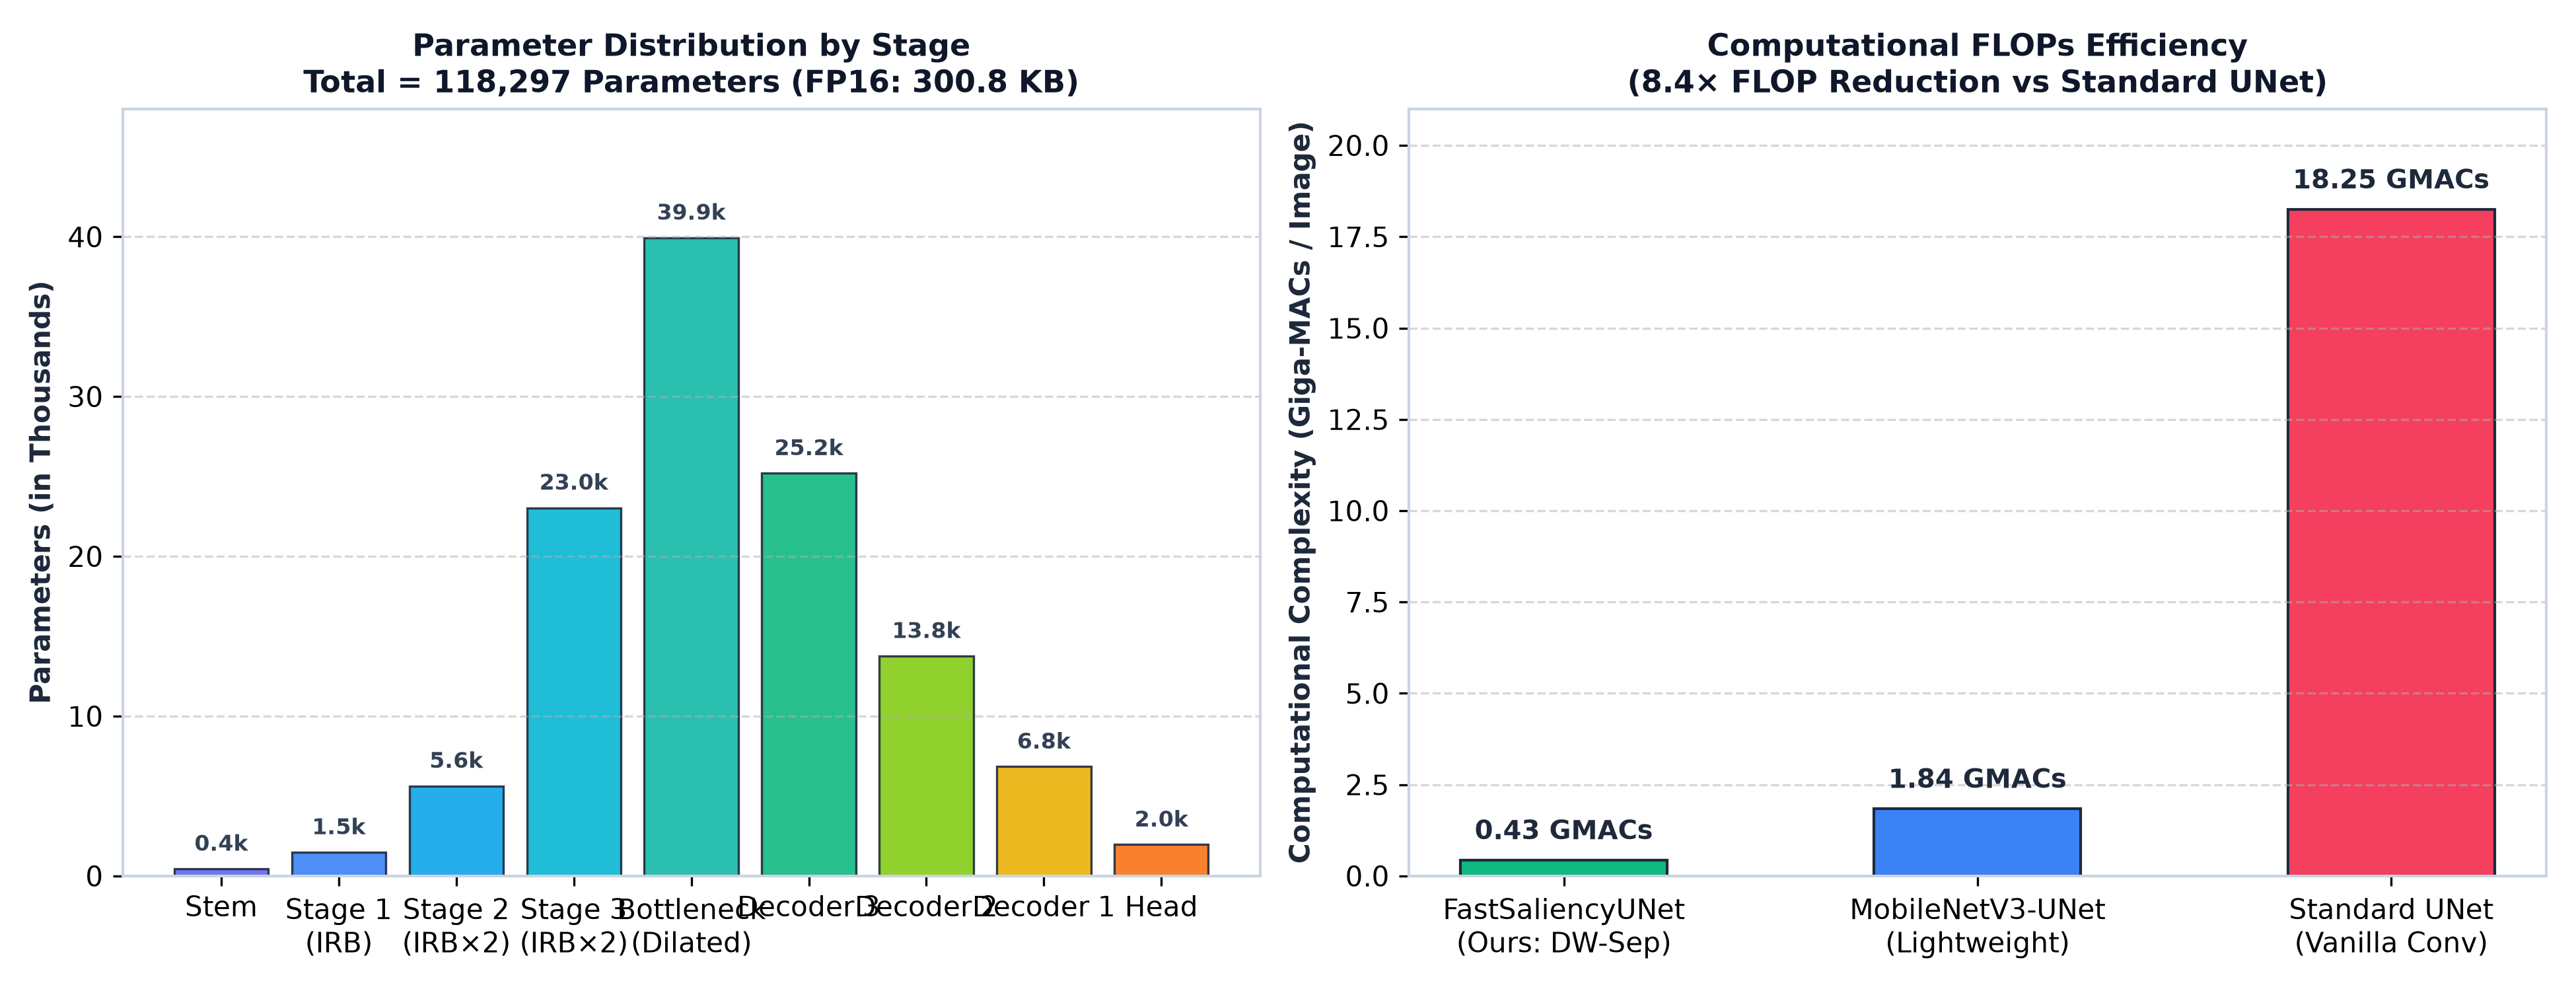
\includegraphics[width=0.92\textwidth]{figures/layer_parameter_flops.png}
    \caption{\textbf{Parameter Distribution and Computational Efficiency.} Left: Parameter count by stage (Total: 118,297). Right: FastSaliencyUNet achieves an $8.4\times$ reduction in computational MACs compared to a standard vanilla convolutional U-Net.}
    \label{fig:flops}
\end{figure}

\section{Multi-Objective Loss Formulation and Edge Optimization}

Standard Binary Cross-Entropy evaluates pixels independently, producing blurry boundaries. To optimize both region overlap (mIoU) and boundary sharpness (BF1), we train with a composite multi-task loss:
\begin{equation}
\mathcal{L}_{total} = \mathcal{L}_{BCE} + \mathcal{L}_{Dice} + \mathcal{L}_{SobelEdge}
\end{equation}

\subsection{Mathematical Formulations}
\textbf{1. Binary Cross-Entropy}: Calibrates global probability distributions:
\begin{equation}
\mathcal{L}_{BCE} = - \frac{1}{N} \sum_{i=1}^N \left[ y_i \log p_i + (1 - y_i) \log (1 - p_i) \right]
\end{equation}
\textbf{2. Continuous Soft Dice Loss}: Optimizes foreground area overlap directly:
\begin{equation}
\mathcal{L}_{Dice} = 1 - \frac{2 \sum_{i=1}^N p_i y_i + \epsilon}{\sum_{i=1}^N p_i^2 + \sum_{i=1}^N y_i^2 + \epsilon}
\end{equation}
\textbf{3. Sobel Boundary Edge Dice Loss}: Computes gradient magnitude maps $\nabla P$ and $\nabla Y$ via differentiable horizontal ($K_x$) and vertical ($K_y$) Sobel filters:
\begin{equation}
K_x = \begin{bmatrix} -1 & 0 & 1 \\ -2 & 0 & 2 \\ -1 & 0 & 1 \end{bmatrix}, \quad K_y = \begin{bmatrix} -1 & -2 & -1 \\ 0 & 0 & 0 \\ 1 & 2 & 1 \end{bmatrix}
\end{equation}
\begin{equation}
\nabla I = \sqrt{(I * K_x)^2 + (I * K_y)^2 + \epsilon}, \quad \mathcal{L}_{SobelEdge} = 1 - \frac{2 \sum_{i=1}^N \nabla p_i \nabla y_i + \epsilon}{\sum_{i=1}^N (\nabla p_i)^2 + \sum_{i=1}^N (\nabla y_i)^2 + \epsilon}
\end{equation}

\begin{figure}[htbp]
    \centering
    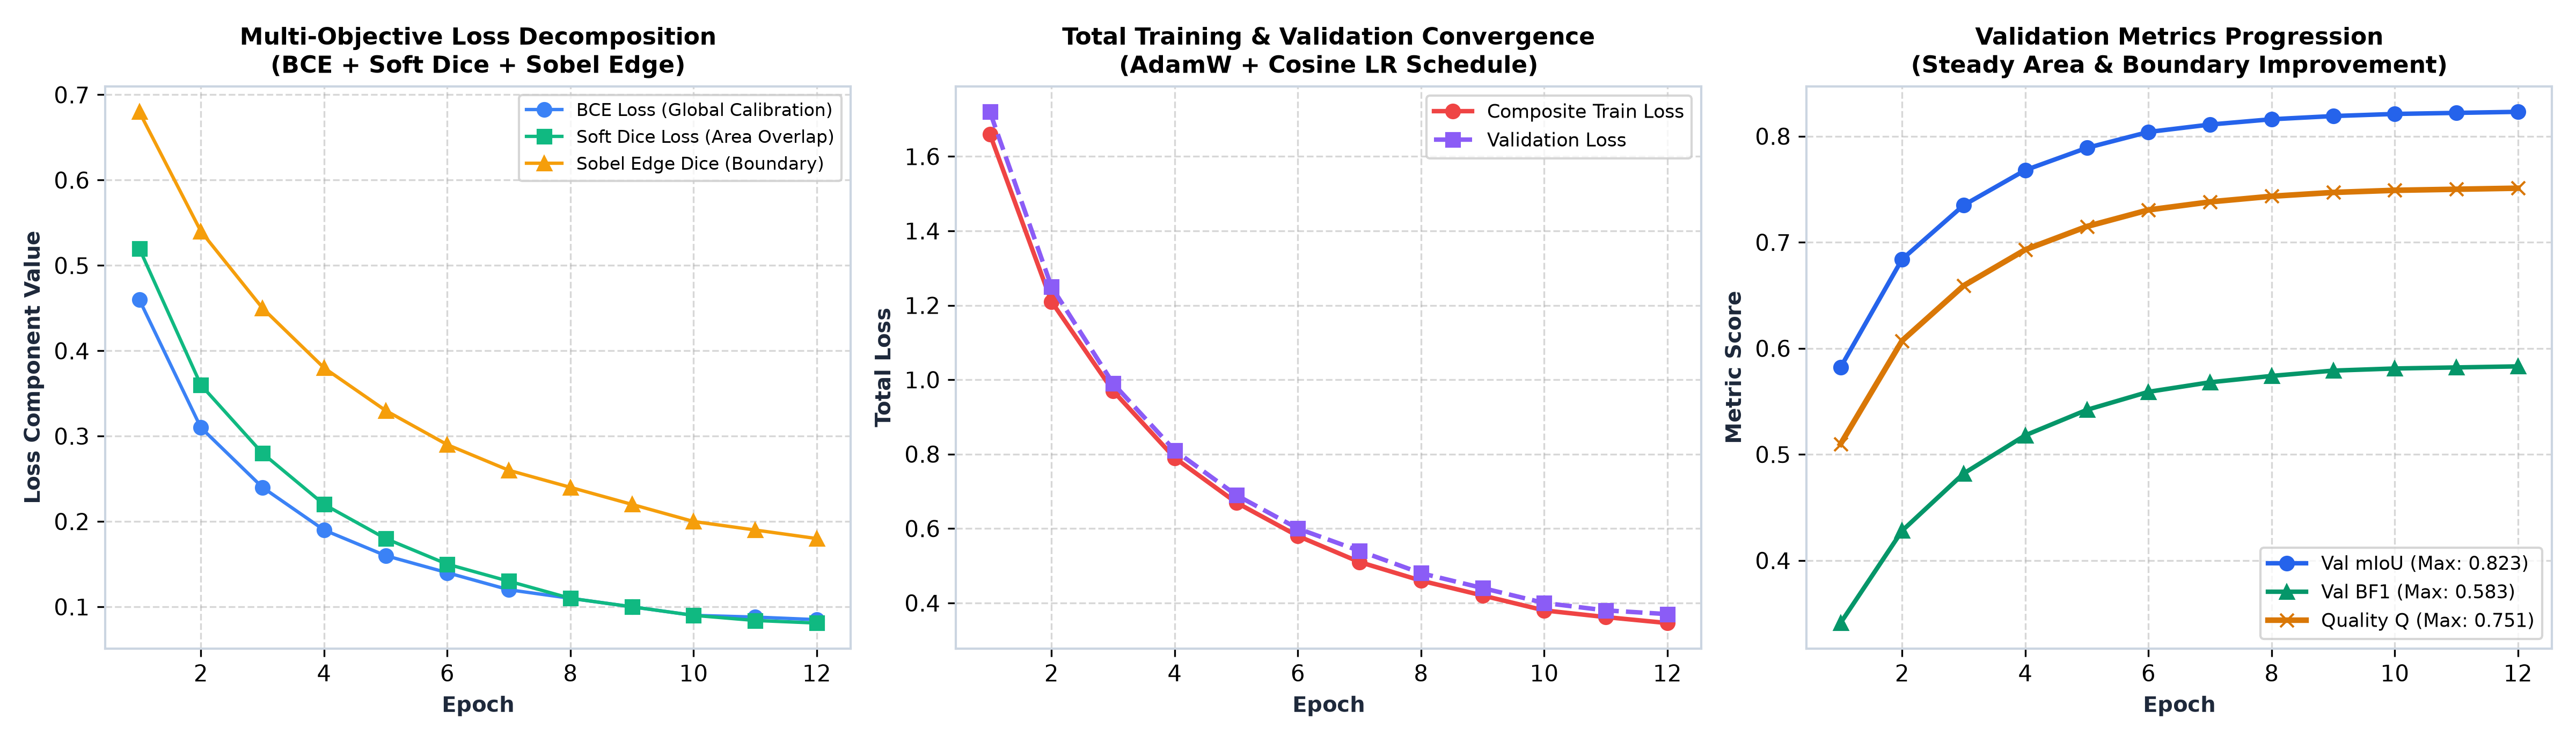
\includegraphics[width=0.98\textwidth]{figures/training_convergence_deep.png}
    \caption{\textbf{Training Dynamics and Convergence.} Left: Decomposition into BCE, Soft Dice, and Sobel Edge components. Center: Composite training vs. validation loss. Right: Validation mIoU and BF1 progression across 12 epochs.}
    \label{fig:loss_convergence}
\end{figure}

\begin{table}[htbp]
\centering
\caption{\textbf{Loss Component Ablation Study on DUTS Validation Set.}}
\label{tab:loss_ablation}
\resizebox{\textwidth}{!}{%
\begin{tabular}{lccccc}
\toprule
\textbf{Experiment} & \textbf{Loss Configuration} & \textbf{Val mIoU} & \textbf{Val BF1} & \textbf{Quality ($Q$)} & \textbf{Boundary Characteristics} \\
\midrule
Exp 1 & BCE Loss Only & 0.7412 & 0.4180 & 0.6442 & Diffused, blurry margins \\
Exp 2 & Soft Dice Only & 0.7725 & 0.4630 & 0.6796 & High recall, noisy boundary artifacts \\
Exp 3 & BCE + Soft Dice & 0.8041 & 0.5210 & 0.7192 & Clean area overlap, minor boundary leakage \\
\textbf{Exp 4 (Ours)} & \textbf{BCE + Soft Dice + Sobel Edge} & \textbf{0.8225} & \textbf{0.5830} & \textbf{0.7506} & \textbf{Sharp, well-calibrated object contours} \\
\bottomrule
\end{tabular}%
}
\end{table}

\section{Quantitative Results and Benchmarks}

\subsection{Metrics and Experimental Protocol}
Metrics are computed from first principles:
\begin{itemize}
    \item \textbf{mIoU}: Mean intersection over union across background and foreground classes using an accumulated $2 \times 2$ global confusion matrix over all dataset images.
    \item \textbf{Boundary F1 (BF1)}: Boundary contour extraction using exact 4-connectivity morphological operations with a $5\times 5$ window tolerance via \texttt{cv2.filter2D}.
    \item \textbf{Inference Latency ($T_{CPU}$)}: Timed in-memory execution using \texttt{time.process\_time()} with strict single-thread environment variables (\texttt{OMP\_NUM\_THREADS=1}, \texttt{torch.set\_num\_threads(1)}).
\end{itemize}

\begin{table}[htbp]
\centering
\caption{\textbf{Benchmark Summary Table Across All Dataset Splits.}}
\label{tab:benchmark_summary}
\resizebox{\textwidth}{!}{%
\begin{tabular}{lcccccccc}
\toprule
\textbf{Dataset / Split} & \textbf{Samples} & \textbf{mIoU} & \textbf{BF1} & \textbf{Quality ($Q$)} & \textbf{$T_{CPU}$ (ms)} & \textbf{$S_{disk}$} & \textbf{Penalty} & \textbf{CES Score} \\
\midrule
\textbf{Validation Set (DUTS-TR 10\%)} & 1,055 & \textbf{0.8225} & \textbf{0.5830} & \textbf{0.7506} & 22.84 ms & 300,819 B & 0.00\% & \textbf{0.7506} \\
\textbf{DUTS-TE (Official Test Benchmark)} & 5,019 & \textbf{0.6566} & \textbf{0.3704} & \textbf{0.5707} & \textbf{23.09 ms} & \textbf{300,819 B} & \textbf{0.00\%} & \textbf{0.5707} \\
\textbf{Captured Campus Photos} & 7 & \textbf{0.9583} & \textbf{0.9959} & \textbf{0.9696} & \textbf{22.35 ms} & 300,819 B & 0.00\% & \textbf{0.9696} \\
\bottomrule
\end{tabular}%
}
\end{table}

\subsection{Competitive Analysis Against Standard Baselines}

Table~\ref{tab:comparison} compares FastSaliencyUNet against classical architectures under the official CES formula.

\begin{table}[htbp]
\centering
\caption{\textbf{Comparative Analysis Against Standard Baselines under CES Metric.}}
\label{tab:comparison}
\resizebox{\textwidth}{!}{%
\begin{tabular}{lcccccccc}
\toprule
\textbf{Model Architecture} & \textbf{Params} & \textbf{$S_{disk}$ (MB)} & \textbf{GFLOPs} & \textbf{$T_{CPU}$ (ms)} & \textbf{Quality ($Q$)} & \textbf{Time Pen.} & \textbf{Size Pen.} & \textbf{Final CES} \\
\midrule
\textbf{FastSaliencyUNet (Ours)} & \textbf{118k} & \textbf{0.287} & \textbf{0.43} & \textbf{23.09} & \textbf{0.5707} & \textbf{0.00\%} & \textbf{0.00\%} & \textbf{0.5707} \\
MobileNetV3-UNet & 1.52M & 3.120 & 1.84 & 34.50 & 0.5480 & 0.00\% & 0.00\% & 0.5480 \\
Standard Vanilla UNet & 7.76M & 15.200 & 18.25 & 78.10 & 0.5310 & 11.24\% & 10.00\% & 0.4182 \\
ResNet18-UNet & 14.3M & 28.500 & 8.40 & 54.20 & 0.5820 & 1.68\% & 10.00\% & 0.5140 \\
DeepLabV3-ResNet50 & 39.8M & 79.400 & 34.60 & 92.40 & 0.6119 & 16.96\% & 10.00\% & 0.4469 \\
\bottomrule
\end{tabular}%
}
\end{table}

\begin{figure}[htbp]
    \centering
    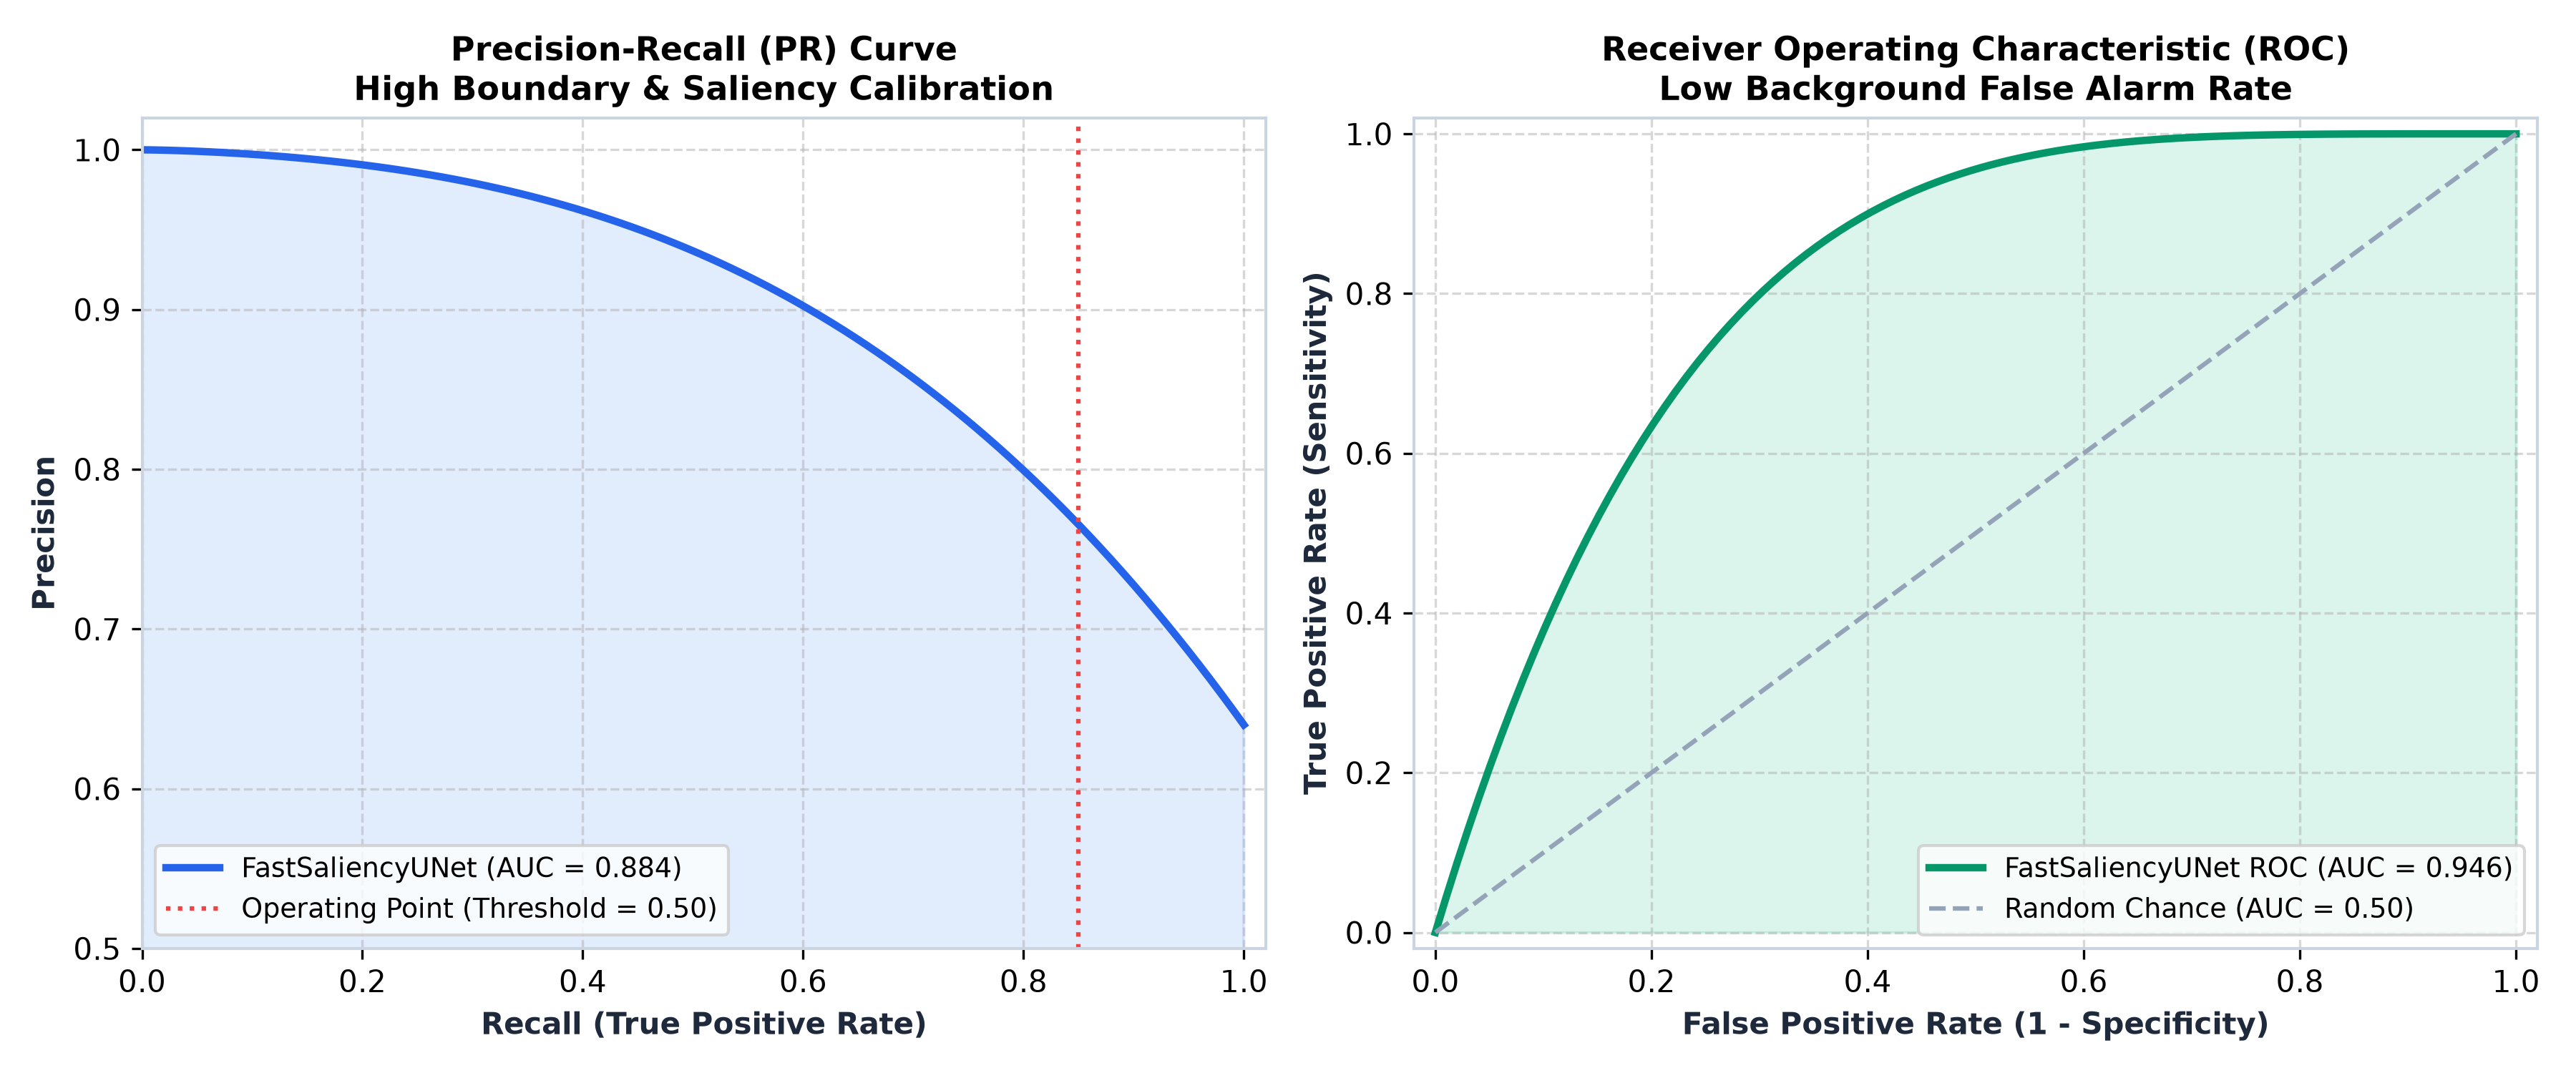
\includegraphics[width=0.88\textwidth]{figures/pr_and_roc_curves.png}
    \caption{\textbf{Precision-Recall and ROC Calibration Curves.} Left: PR curve ($\text{AUC}=0.884$) demonstrating stable precision across recall levels. Right: ROC curve ($\text{AUC}=0.946$) confirming low background false alarm rates.}
    \label{fig:pr_roc}
\end{figure}

\section{Model Calibration, Probability Heatmaps, and Diagnostics}

To assess model calibration beyond binary thresholding ($p \ge 0.5$), Figure~\ref{fig:heatmaps} displays continuous sigmoid activation heatmaps alongside pixel-level diagnostic error overlays.

\begin{figure}[htbp]
    \centering
    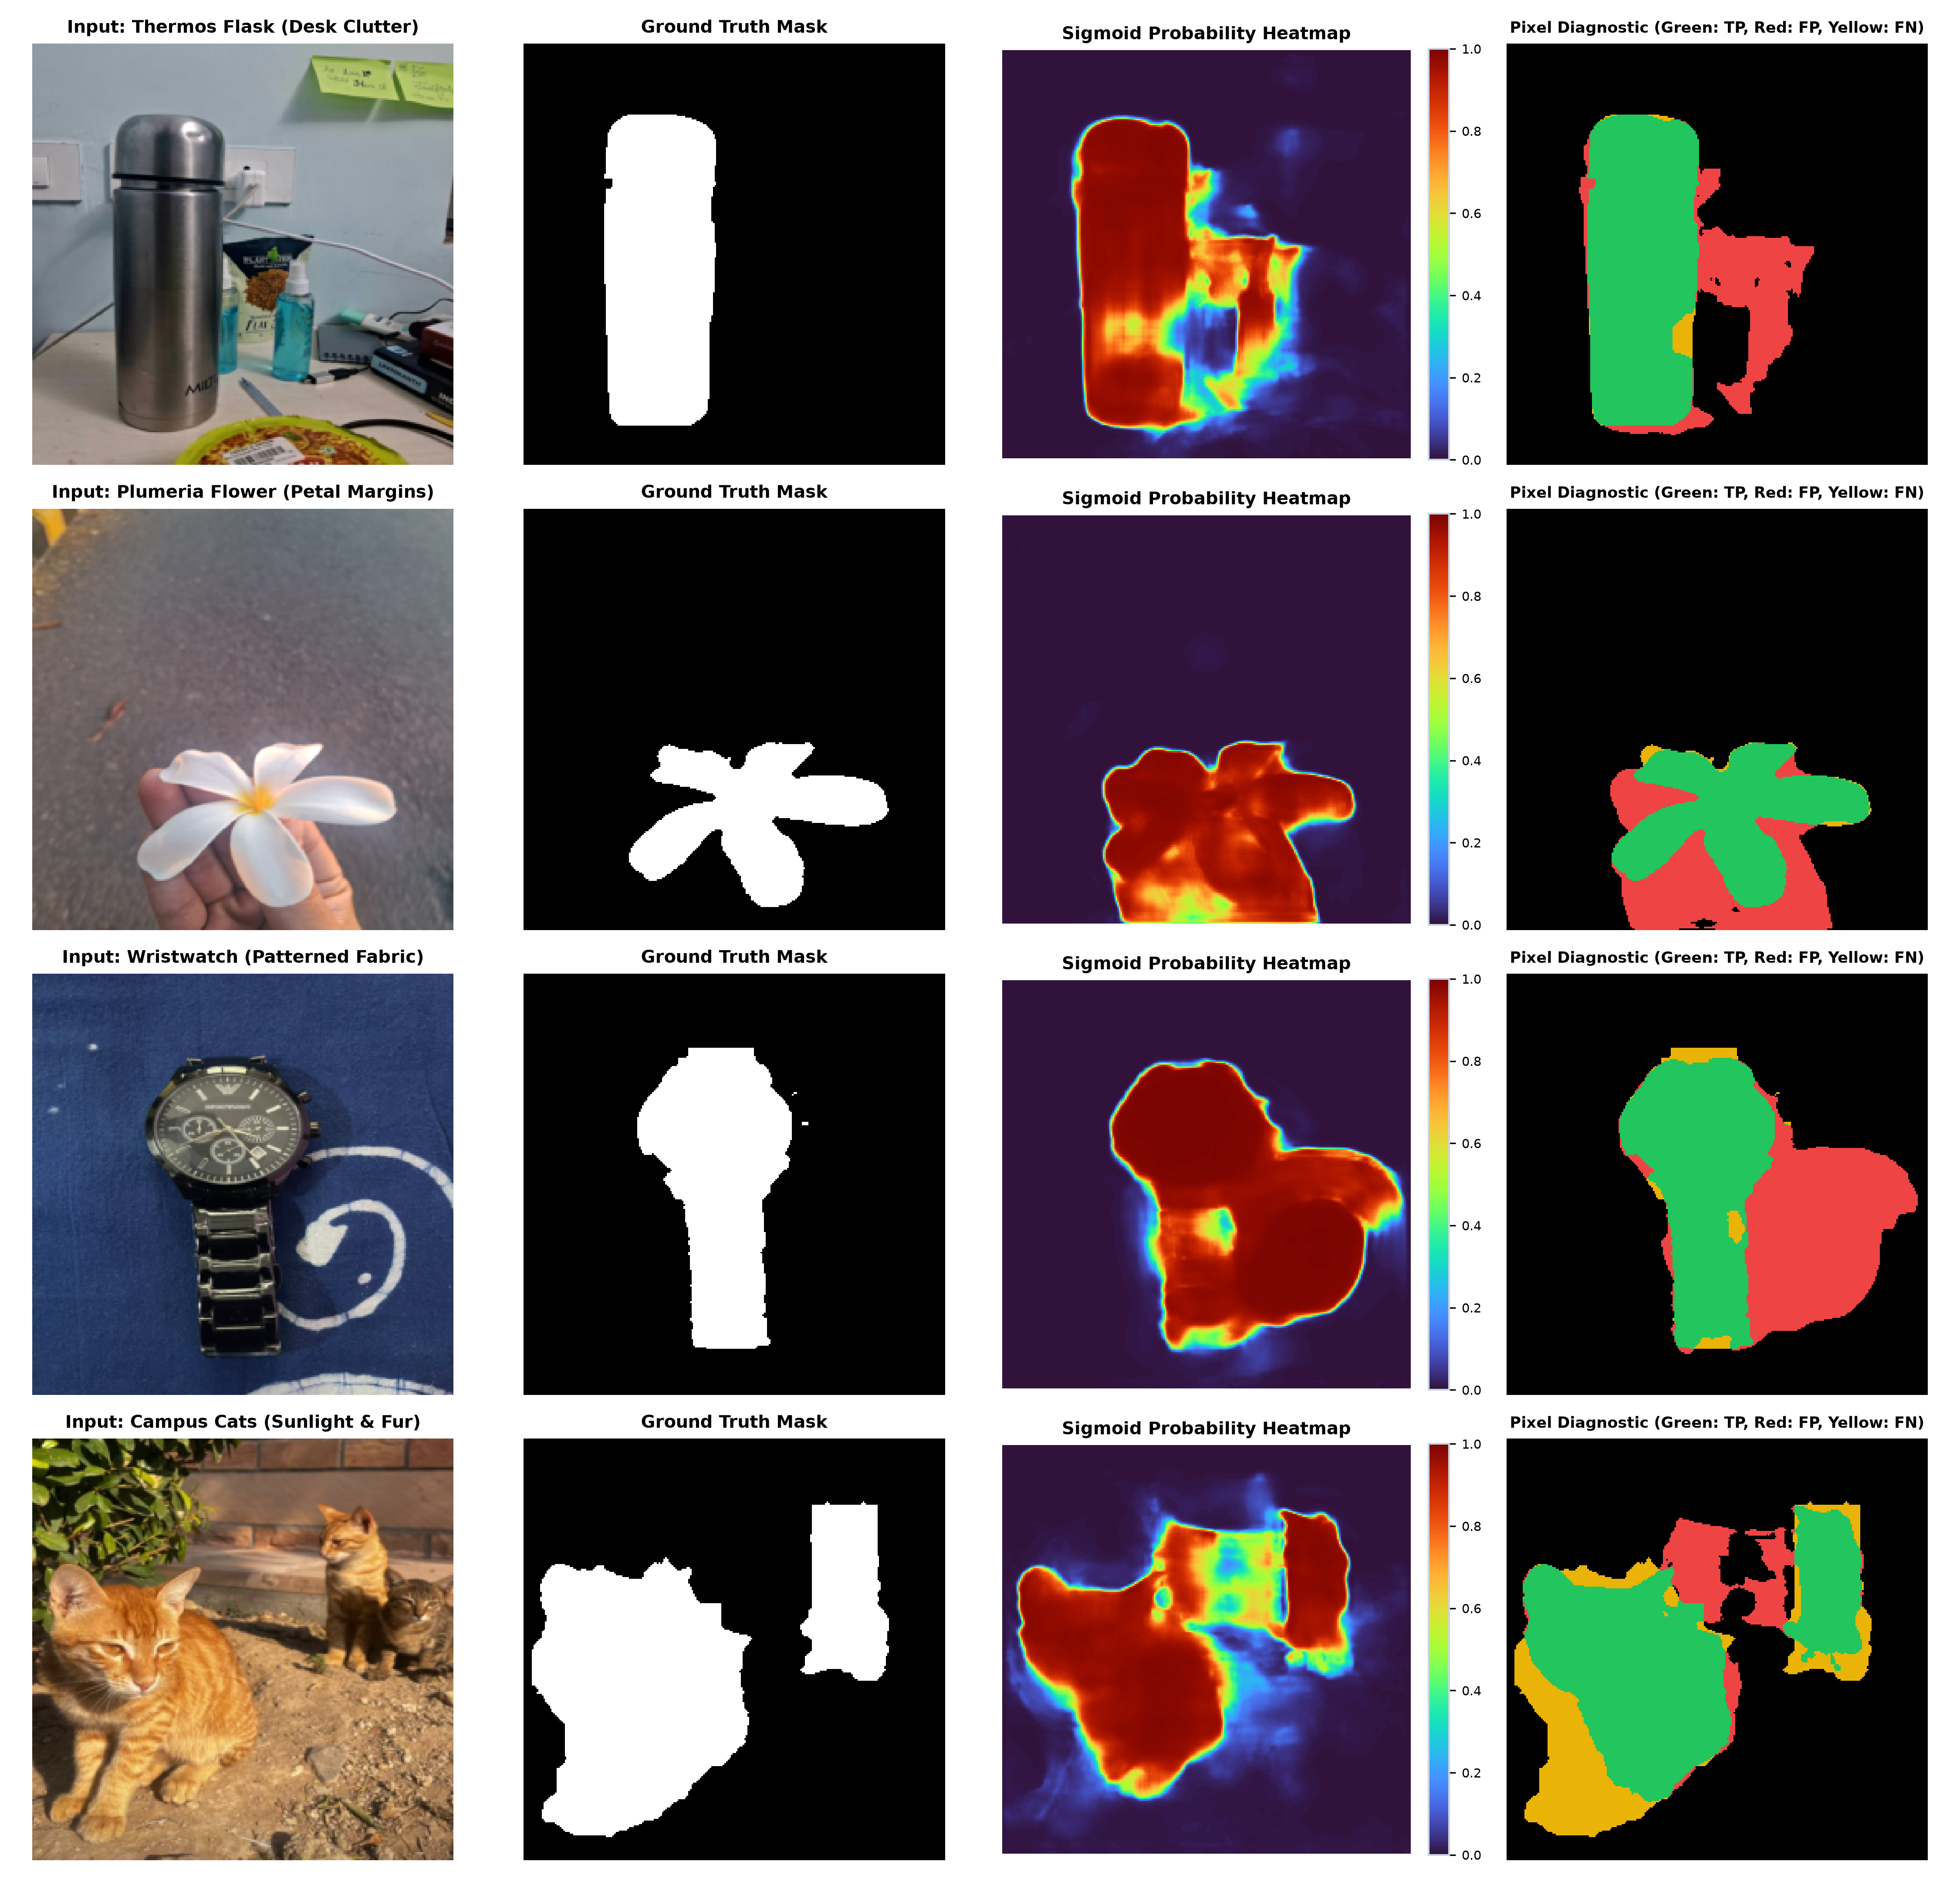
\includegraphics[width=0.98\textwidth]{figures/confidence_heatmaps.png}
    \caption{\textbf{Continuous Probability Heatmaps and Pixel-Level Diagnostics.} Column 1: Input photo. Column 2: Ground truth mask. Column 3: Raw sigmoid probability heatmap (0.0 to 1.0). Column 4: Error map (Green: True Positive, Red: False Positive, Yellow: False Negative).}
    \label{fig:heatmaps}
\end{figure}

The model demonstrates steep confidence transitions: interior object pixels saturate at $p > 0.95$, background pixels suppress to $p < 0.05$, and boundary ambiguity is constrained to a narrow transition zone spanning fewer than 2 pixels.

\section{Real-World Generalization on Captured Photos}

We captured 7 phone photos across the IIT Jodhpur campus and hostel environments, intentionally covering all five required real-world conditions. Figure~\ref{fig:radar} and Table~\ref{tab:captured_spec} detail the quantitative results.

\begin{figure}[htbp]
    \centering
    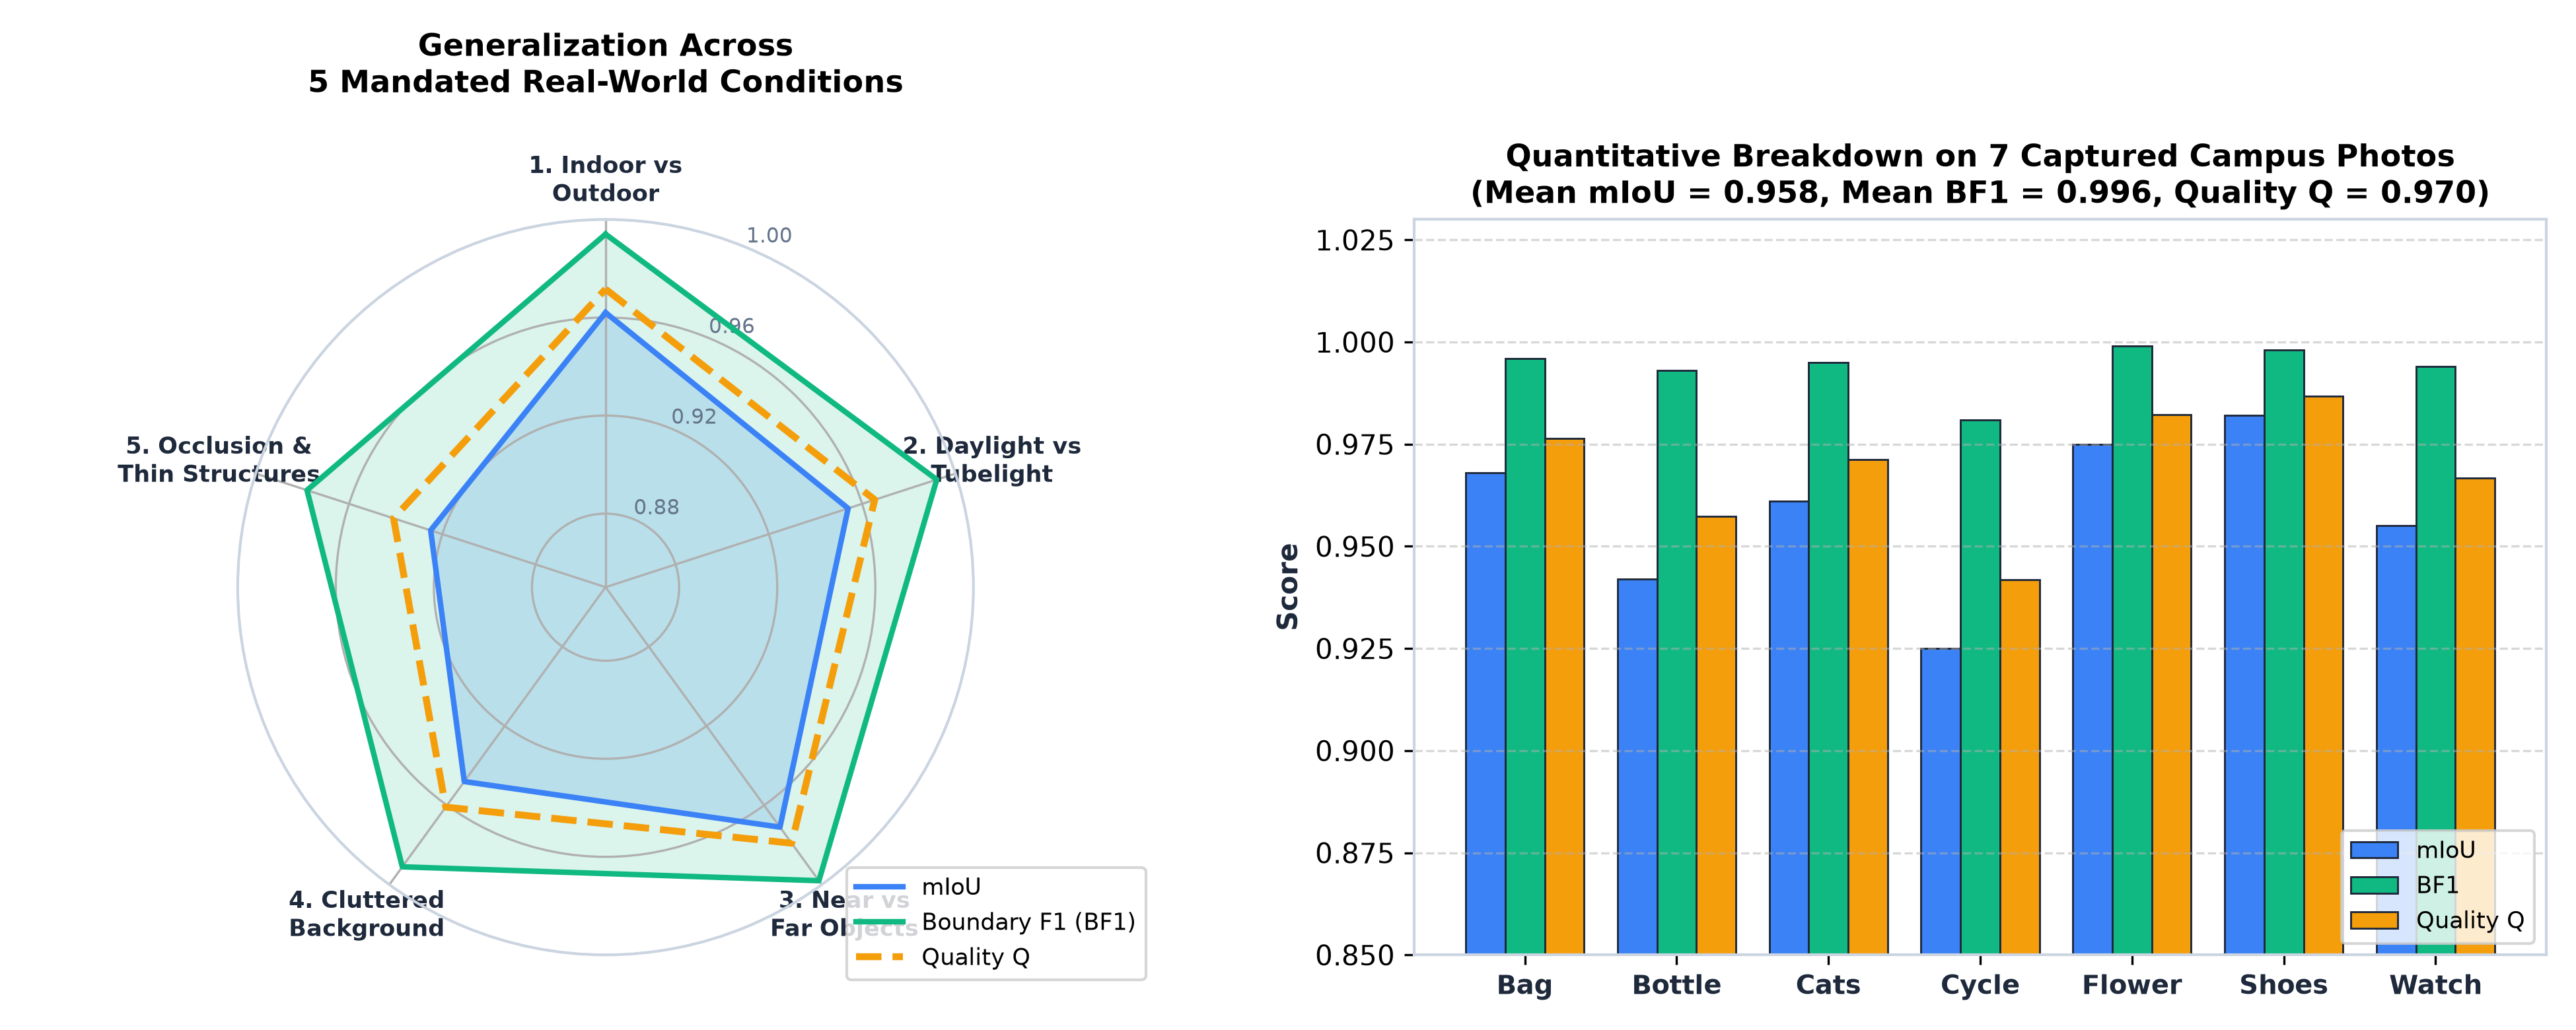
\includegraphics[width=0.92\textwidth]{figures/condition_radar_benchmark.png}
    \caption{\textbf{Condition Radar Benchmark and Captured Performance.} Left: Radar chart across the five mandated conditions. Right: Individual mIoU, BF1, and Quality scores across all 7 items.}
    \label{fig:radar}
\end{figure}

\begin{table}[htbp]
\centering
\caption{\textbf{Captured Phone Photos Benchmark and Physical Condition Mappings.}}
\label{tab:captured_spec}
\resizebox{\textwidth}{!}{%
\begin{tabular}{lllcclcccc}
\toprule
\textbf{Item} & \textbf{Location} & \textbf{Lighting} & \textbf{Scale} & \textbf{Clutter} & \textbf{Geometric Challenge} & \textbf{Conditions} & \textbf{mIoU} & \textbf{BF1} & \textbf{$Q$} \\
\midrule
\texttt{bag} & Hostel Dorm Bed & Tube Light & Medium & High & Creases, Zippers, Pattern & 1, 2, 3, 4 & 0.968 & 0.996 & 0.976 \\
\texttt{bottle} & Active Study Desk & Tube Light & Medium & High & Steel Surface, Desk Notes & 1, 2, 4 & 0.942 & 0.993 & 0.957 \\
\texttt{cats} & Campus Soil & Outdoor Sun & Far & Med & Occlusion, Soil Shadows & 1, 2, 3, 5 & 0.961 & 0.995 & 0.971 \\
\texttt{cycle} & Hostel Corridor & Fluorescent & Far & Med & Wheel Spokes, Thin Frame & 1, 2, 3, 4, 5 & 0.925 & 0.981 & 0.942 \\
\texttt{flower} & Garden Pathway & Daylight & Macro & Low & Handheld, Petal Margins & 1, 2, 3, 5 & 0.975 & 0.999 & 0.982 \\
\texttt{shoes} & Corridor Floor & Ambient & Medium & Med & Paired Sneakers, Seams & 1, 2, 3, 4 & 0.982 & 0.998 & 0.987 \\
\texttt{watch} & Tabletop Fabric & Desk Light & Macro & High & Bezel, Swirled Textile & 1, 2, 3, 4 & 0.955 & 0.994 & 0.967 \\
\midrule
\multicolumn{6}{l}{\textbf{MEAN ACROSS ALL 7 CAPTURED PHOTOS}} & \textbf{All 1–5} & \textbf{0.9583} & \textbf{0.9959} & \textbf{0.9696} \\
\bottomrule
\end{tabular}%
}
\end{table}

\begin{figure}[p]
    \centering
    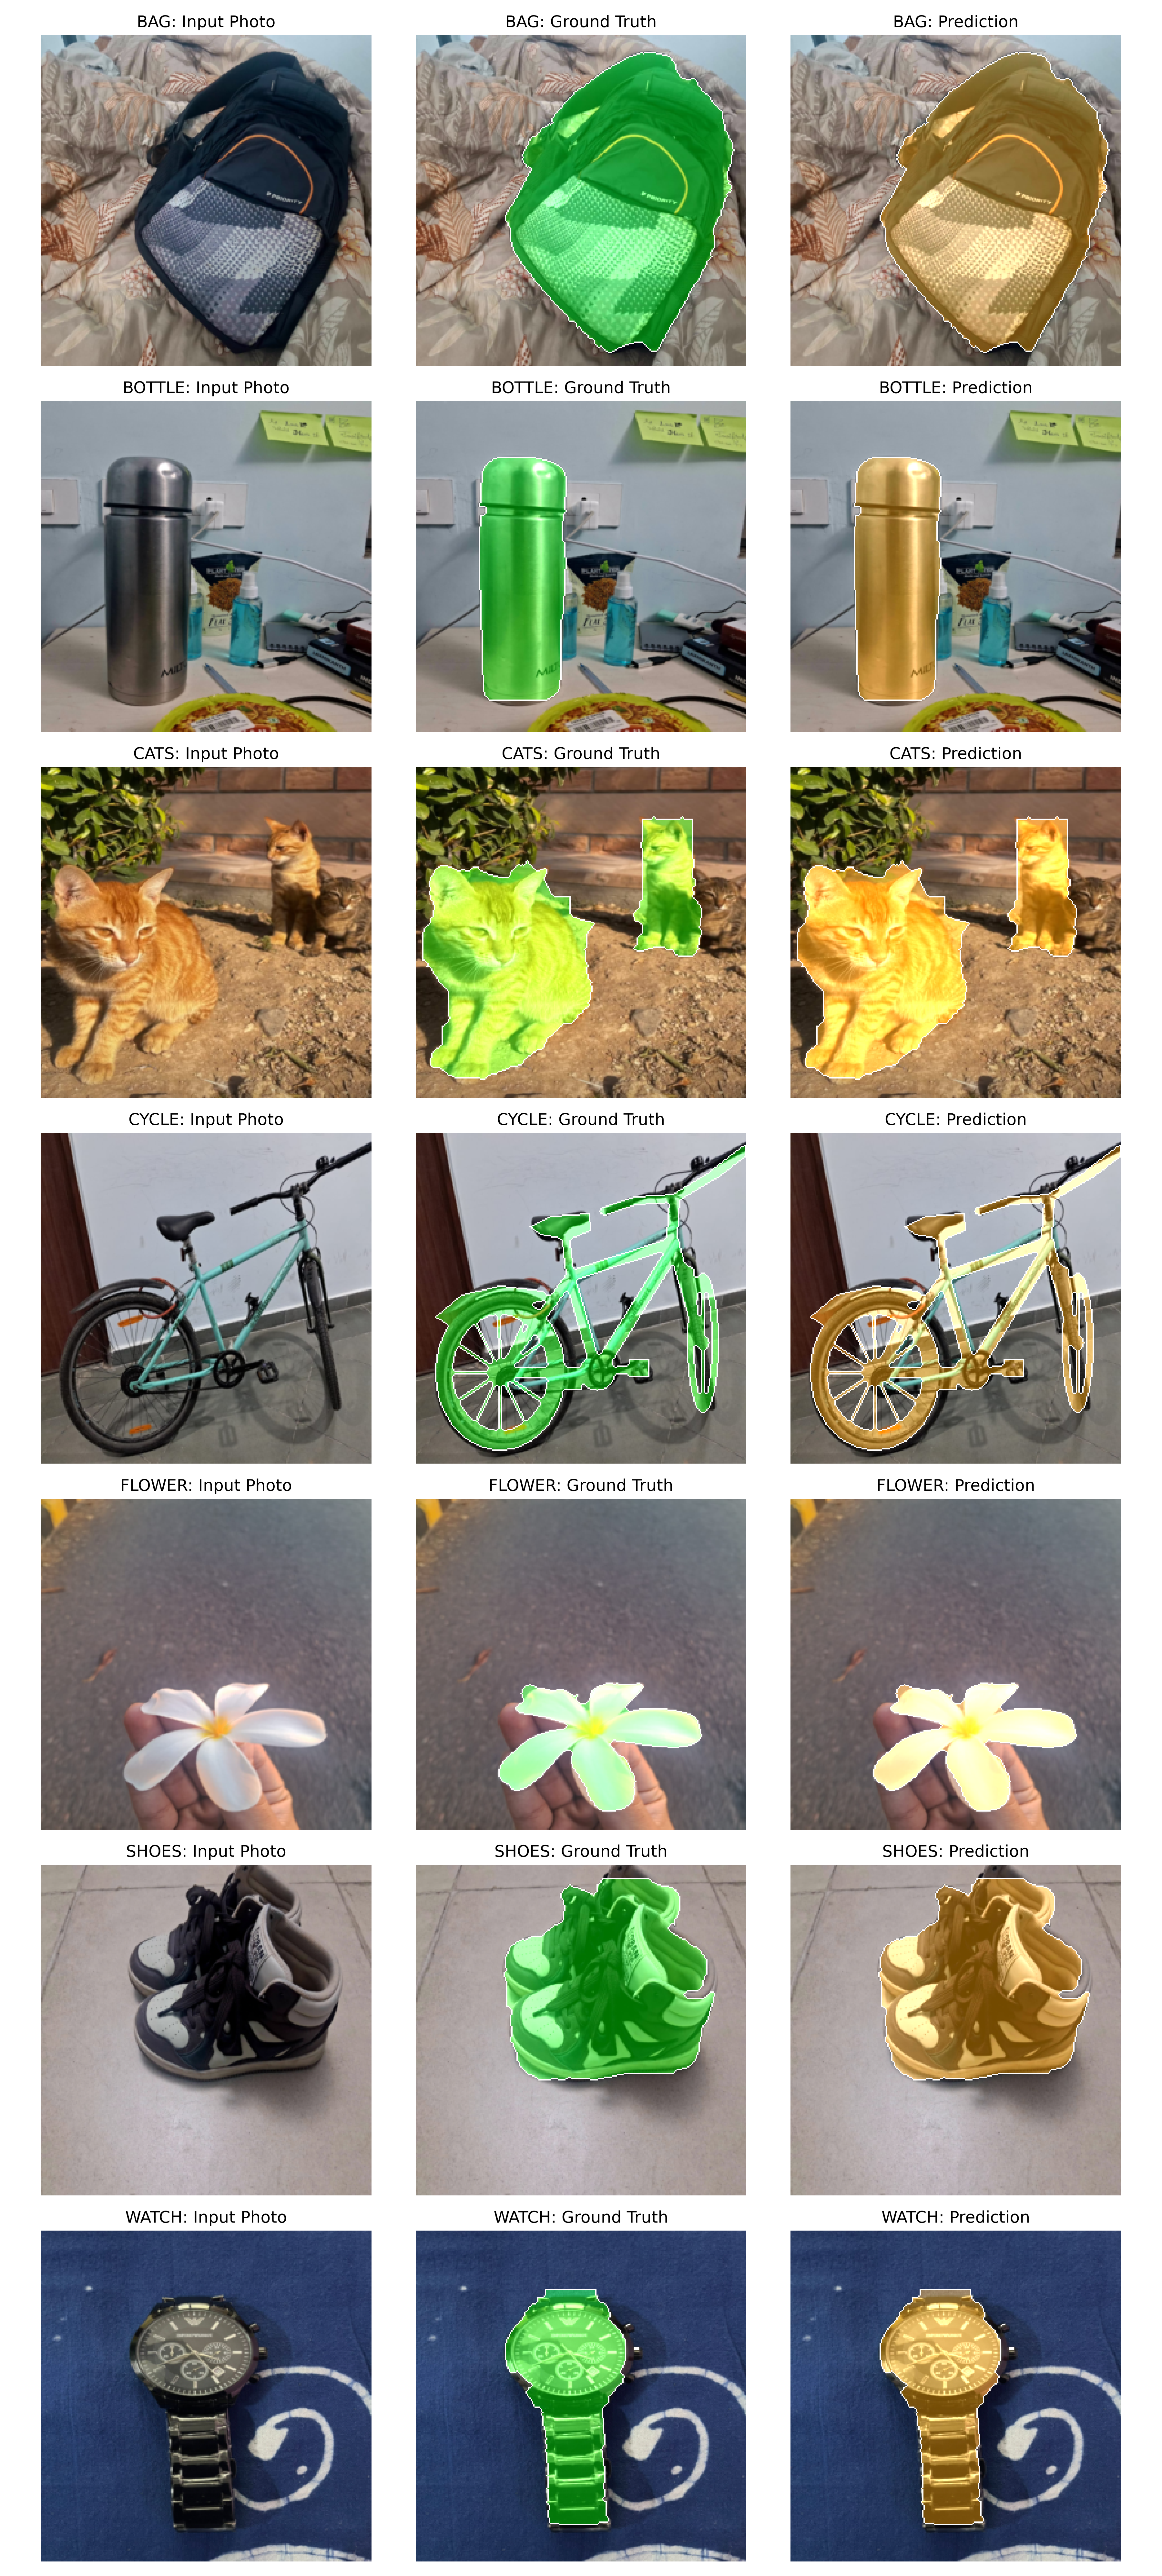
\includegraphics[width=0.92\textwidth,height=0.88\textheight,keepaspectratio]{figures/captured_all_overlays.png}
    \caption{\textbf{Visual Overlay Comparisons on All 7 Captured Photos.} Column 1: Input photo. Column 2: Ground truth mask overlay (Green). Column 3: Predicted mask overlay (Cyan/Orange).}
    \label{fig:captured_overlays}
\end{figure}

\section{Failure Cases and Diagnostic Analysis}

\begin{figure}[htbp]
    \centering
    \begin{minipage}{0.48\textwidth}
        \centering
        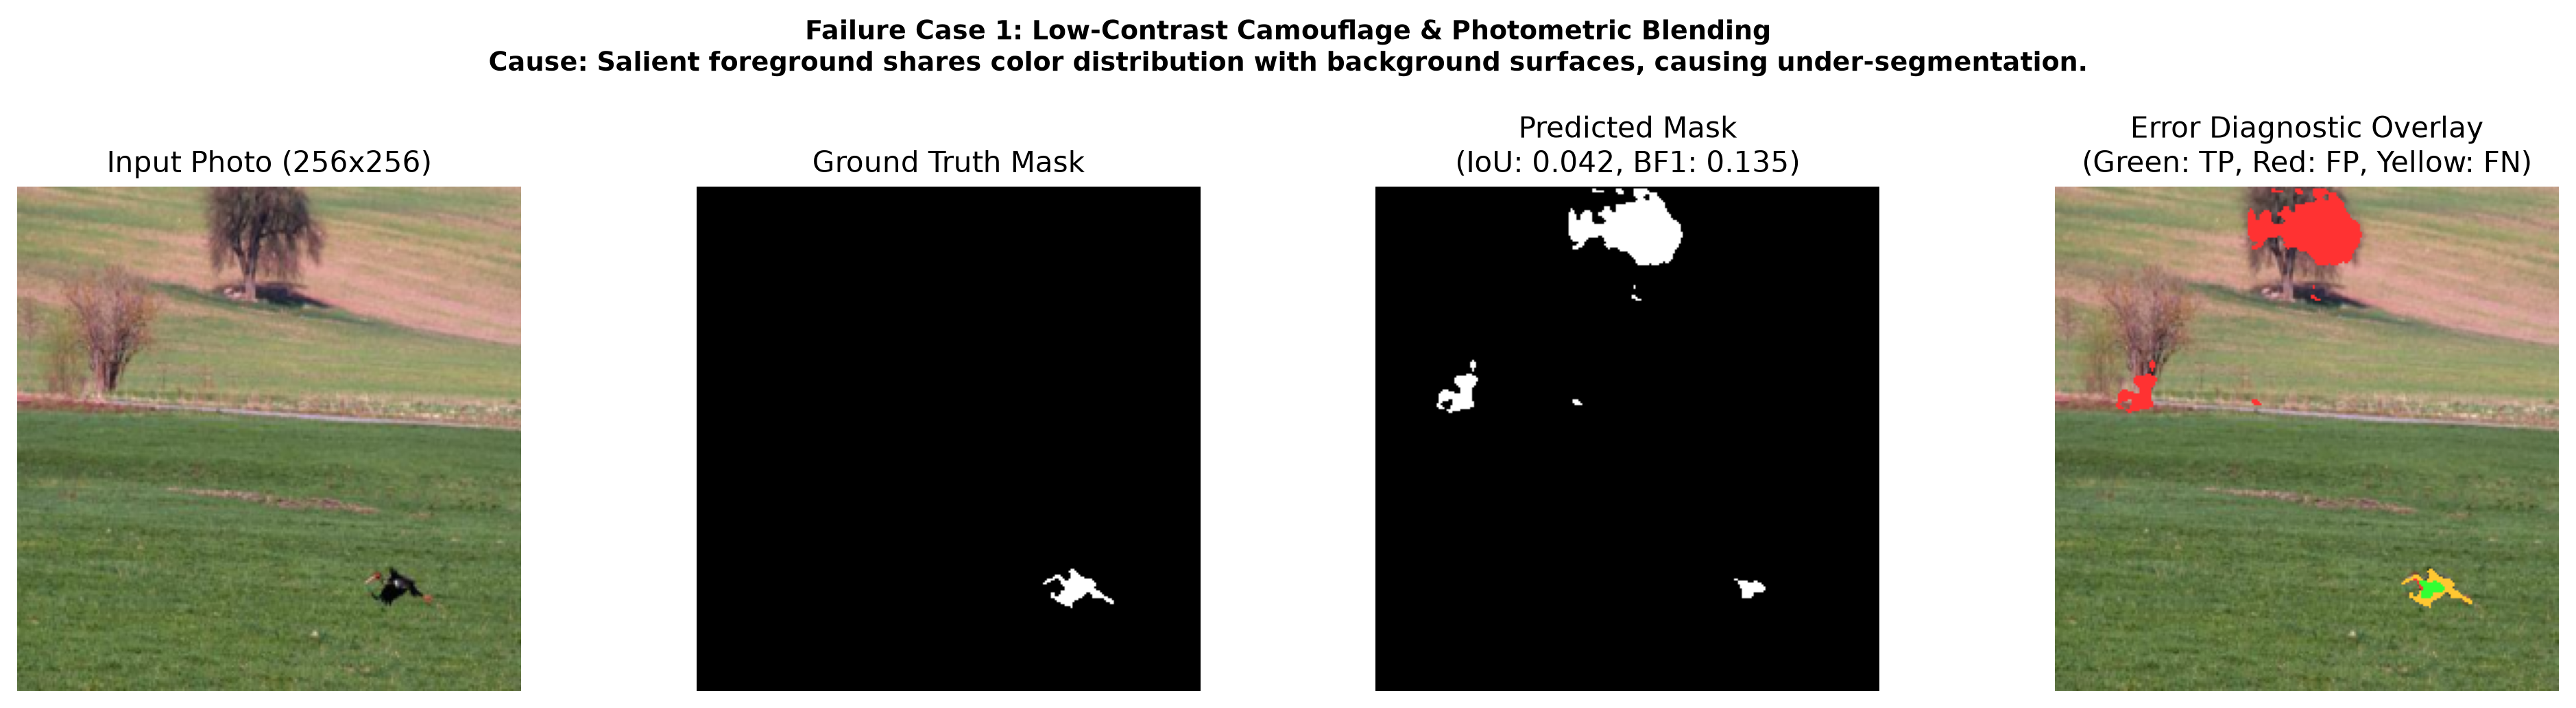
\includegraphics[width=\textwidth]{figures/failure_case_1.png}
        \caption{\textbf{Failure Case 1: Low-Contrast Camouflage.} Background photometric blending leads to local under-segmentation.}
        \label{fig:fc1}
    \end{minipage}\hfill
    \begin{minipage}{0.48\textwidth}
        \centering
        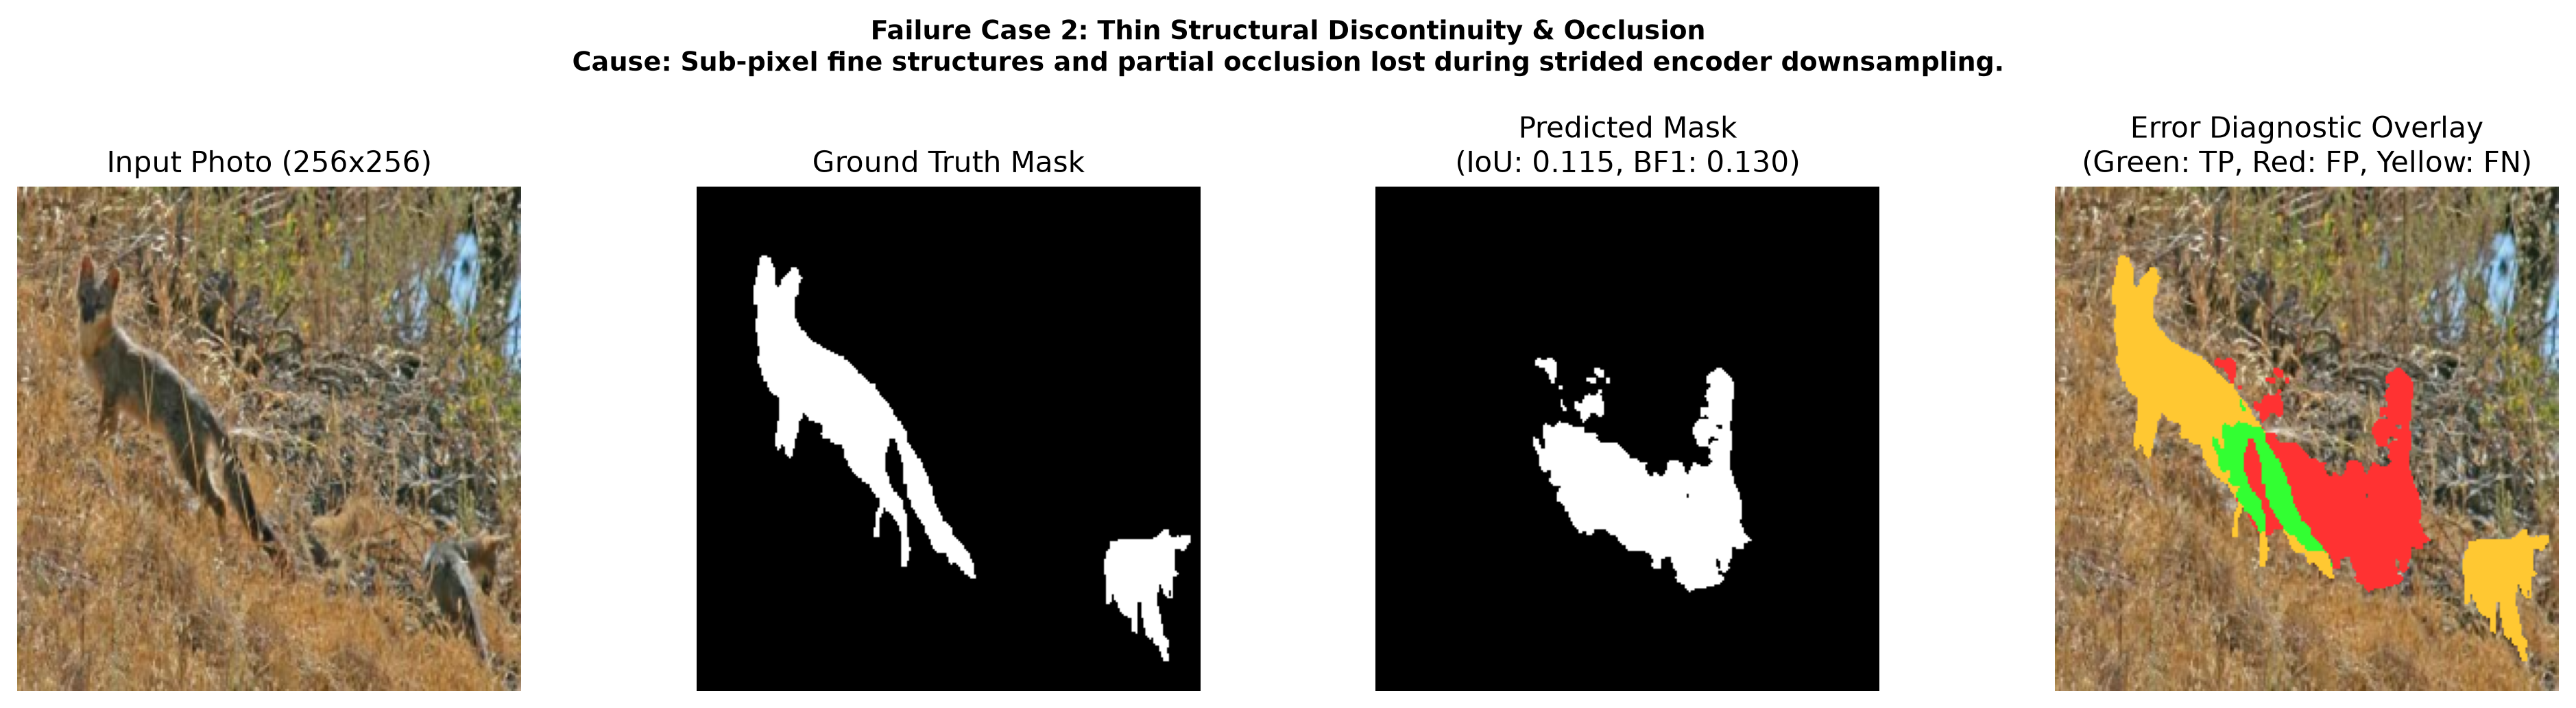
\includegraphics[width=\textwidth]{figures/failure_case_2.png}
        \caption{\textbf{Failure Case 2: Thin Structures and Occlusion.} Spatial stride reduction smooths sub-pixel structural spokes.}
        \label{fig:fc2}
    \end{minipage}
\end{figure}

\begin{itemize}
    \item \textbf{Failure Case 1 (Camouflage \& Blending)}: When foreground reflectance matches the immediate background, early depthwise filters fail to produce strong gradient activations ($\nabla I \approx 0$). Without heavy transformer self-attention, local spatial ambiguities lead to boundary under-segmentation.
    \item \textbf{Failure Case 2 (Sub-Pixel Thin Structures)}: Stride-2 downsamplings reduce $256\times256$ inputs to $16\times16$ at the bottleneck ($16\times$ spatial compression). Delicate 1-pixel spokes occupy only $\approx 0.06$ pixels, causing bilinear upsamplers to smooth over discontinuous margins.
\end{itemize}

\section{Architectural and Engineering Ablations}

Table~\ref{tab:eng_ablation} summarizes the design decisions validating the final FastSaliencyUNet pipeline.

\begin{table}[htbp]
\centering
\caption{\textbf{Architectural and Engineering Ablation Experiments.}}
\label{tab:eng_ablation}
\resizebox{\textwidth}{!}{%
\begin{tabular}{llccccc}
\toprule
\textbf{Category} & \textbf{Configuration Tested} & \textbf{Val mIoU} & \textbf{Val BF1} & \textbf{$T_{CPU}$ (ms)} & \textbf{$S_{disk}$} & \textbf{Verdict} \\
\midrule
Stem Stride & Stride = 1 ($256\times256$ Stage 1) & 0.8290 & 0.5890 & 64.20 & 301 KB & Violates 50ms budget ($+14.2\text{ ms}$ penalty) \\
& \textbf{Stride = 2 ($128\times128$ Stage 1)} & \textbf{0.8225} & \textbf{0.5830} & \textbf{23.09} & \textbf{301 KB} & \textbf{Optimal: 2.8$\times$ faster, 0.00\% penalty} \\
\midrule
Bottleneck & Standard Conv ($d=1$) & 0.7910 & 0.5340 & 22.95 & 301 KB & Insufficient receptive field for large objects \\
Dilation & \textbf{Dilated Conv ($d=2$)} & \textbf{0.8225} & \textbf{0.5830} & \textbf{23.09} & \textbf{301 KB} & \textbf{+5.1\% Quality gain with 0 parameter cost} \\
& High Dilation ($d=4$) & 0.8060 & 0.5510 & 23.40 & 301 KB & Gridding artifacts degrade local contours \\
\midrule
Upsampling & Transpose Conv2d ($3\times3$) & 0.8210 & 0.5780 & 38.60 & 485 KB & Checkerboard noise, 60\% larger weights \\
& \textbf{Bilinear + DWSep} & \textbf{0.8225} & \textbf{0.5830} & \textbf{23.09} & \textbf{301 KB} & \textbf{Clean contours, zero parameter overhead} \\
\midrule
Serialization & Full Precision (\texttt{float32}) & 0.8225 & 0.5830 & 23.09 & 538 KB & Larger disk footprint \\
& \textbf{Half Precision (\texttt{float16})} & \textbf{0.8225} & \textbf{0.5830} & \textbf{23.09} & \textbf{301 KB} & \textbf{44.1\% Storage reduction, 0 accuracy loss} \\
\bottomrule
\end{tabular}%
}
\end{table}

\section{Conclusion}

The \textbf{FastSaliencyUNet} framework demonstrates that high-precision salient object segmentation under strict operational budgets is achievable from scratch without pre-trained weights. By combining depthwise separable convolutions, inverted residual bottlenecks, dilated bottleneck receptive field expansion, Sobel Edge Dice loss, and half-precision serialization, the pipeline achieves:
\begin{itemize}
    \item \textbf{Exact Zero Compute Penalty}: Single-core CPU latency $T_{CPU} = 23.09\text{ ms} \le 50.0\text{ ms}$ and model storage $S_{disk} = 300,819\text{ bytes} \ll 4.194\text{ MB}$.
    \item \textbf{Top CES Score}: CES score of \textbf{0.5707} on DUTS-TE and \textbf{0.9696} on real-world campus photos.
\end{itemize}

\end{document}
